\RequirePackage[l2tabu,orthodox]{nag}

\documentclass[headsepline,footsepline,footinclude=false,fontsize=11pt,paper=a4,listof=totoc,bibliography=totoc,BCOR=12mm,DIV=12]{scrbook} % two-sided
%\documentclass[headsepline,footsepline,footinclude=false,oneside,fontsize=11pt,paper=a4,listof=totoc,bibliography=totoc]{scrbook}


\PassOptionsToPackage{table,svgnames,dvipsnames}{xcolor}

\usepackage[utf8]{inputenc}
\usepackage[T1]{fontenc}
\usepackage[sc]{mathpazo}
\usepackage[ngerman,american]{babel}
\usepackage[autostyle]{csquotes}

\usepackage[
backend=biber,
%style=authoryear,
style=alphabetic,
]{biblatex}

\usepackage{graphicx}
\usepackage{scrhack}
\usepackage{acronym}
\usepackage{listings}
\usepackage{lstautogobble}
\usepackage{tikz}
\usepackage{pgfplots}
\usepackage{pgfplotstable}
\usepackage{booktabs}
\usepackage{multirow}
\usepackage{mwe}
\usepackage{comment}
\usepackage{textcomp}
\usepackage{amsmath}
\usepackage{subfig}
\usepackage{textcmds}
\usepackage[final]{microtype}
\usepackage{caption}
\usepackage[hidelinks]{hyperref} % hidelinks removes colored boxes around references and links
\usepackage{verbatim}
\usepackage{cleveref}
\usepackage{xr}
\usepackage{algorithm}
\usepackage{algpseudocode}
\usepackage{algorithmicx}

\addbibresource{bibliography.bib}

%\bibliographystyle{plain}

\setkomafont{disposition}{\normalfont\bfseries} % use serif font for headings
\linespread{1.05} % adjust line spread for mathpazo font

% Add table of contents to PDF bookmarks
\BeforeTOCHead[toc]{{\cleardoublepage\pdfbookmark[0]{\contentsname}{toc}}}

% Define TUM corporate design colors
% Taken from http://portal.mytum.de/corporatedesign/index_print/vorlagen/index_farben
\definecolor{TUMBlue}{HTML}{0065BD}
\definecolor{TUMSecondaryBlue}{HTML}{005293}
\definecolor{TUMSecondaryBlue2}{HTML}{003359}
\definecolor{TUMBlack}{HTML}{000000}
\definecolor{TUMWhite}{HTML}{FFFFFF}
\definecolor{TUMDarkGray}{HTML}{333333}
\definecolor{TUMGray}{HTML}{808080}
\definecolor{TUMLightGray}{HTML}{CCCCC6}
\definecolor{TUMAccentGray}{HTML}{DAD7CB}
\definecolor{TUMAccentOrange}{HTML}{E37222}
\definecolor{TUMAccentGreen}{HTML}{A2AD00}
\definecolor{TUMAccentLightBlue}{HTML}{98C6EA}
\definecolor{TUMAccentBlue}{HTML}{64A0C8}

% Settings for pgfplots
\pgfplotsset{compat=newest}
\pgfplotsset{
  % For available color names, see http://www.latextemplates.com/svgnames-colors
  cycle list={TUMBlue\\TUMAccentOrange\\TUMAccentGreen\\TUMSecondaryBlue2\\TUMDarkGray\\},
}

% Settings for lstlistings
\lstset{%
  basicstyle=\ttfamily,
  columns=fullflexible,
  autogobble,
  keywordstyle=\bfseries\color{TUMBlue},
  stringstyle=\color{TUMAccentGreen}
}


\newcommand*{\getUniversity}{Technical University of Munich}
\newcommand*{\getFaculty}{Software and Systems Engineering}
\newcommand*{\getTitle}{Scraping online documentation of Ardupilot UAV system to generate a knowledge-based causal graph}
\newcommand*{\getTitleGer}{Scraping der Online-Dokumentation des Ardupilot-Drohnensystems zur Generierung eines wissensbasierten Kausalgraphen.}
\newcommand*{\getAuthor}{Robin Borth}
\newcommand*{\getDoctype}{Bachelor's Thesis in Informatics}
\newcommand*{\getSupervisor}{Prof. Dr. Alexander Pretschner}
\newcommand*{\getAdvisor}{Ehsan Zibaei}
\newcommand*{\getSubmissionDate}{15.02.2022}
\newcommand*{\getSubmissionLocation}{Munich}

\begin{document}

    \pagenumbering{alph}
    \begin{titlepage}
  % HACK for two-sided documents: ignore binding correction for cover page.
  % Adapted from Markus Kohm's KOMA-Script titlepage=firstiscover handling.
  % See http://mirrors.ctan.org/macros/latex/contrib/koma-script/scrkernel-title.dtx,
%  \maketitle macro
  \oddsidemargin=\evensidemargin\relax
  \textwidth=\dimexpr\paperwidth-2\evensidemargin-2in\relax
  \hsize=\textwidth\relax

  \centering

  \IfFileExists{logos/tum.pdf}{%
    
\includegraphics[height=20mm]{logos/tum.pdf}
  }{%
    \vspace*{20mm}
  }

  \vspace{5mm}
  {\huge\MakeUppercase{Software and Systems}}\\
  \vspace{2mm}
  {\huge\MakeUppercase{Engineering}}\\

  \vspace{5mm}
  {\large\MakeUppercase{\getUniversity{}}}\\

  \vspace{20mm}
  {\Large \getDoctype{}}

  \vspace{15mm}
  {\huge\bfseries \getTitle{}}

  \vspace{15mm}
  {\LARGE \getAuthor{}}

  \IfFileExists{logos/faculty.pdf}{%
    \vfill{}
    
\includegraphics[height=20mm]{logos/faculty.pdf}
  }{}
\end{titlepage}


    \frontmatter{}

    \begin{titlepage}
  \centering

  \IfFileExists{logos/tum.pdf}{%
    
\includegraphics[height=20mm]{logos/tum.pdf}
  }{%
    \vspace*{20mm}
  }

  \vspace{5mm}
  {\huge\MakeUppercase{\getFaculty{}}}\\

  \vspace{5mm}
  {\large\MakeUppercase{\getUniversity{}}}\\

  \vspace{10mm}
  {\Large \getDoctype{}}

  \vspace{10mm}
  {\huge\bfseries \getTitle{} \par}

  \vspace{10mm}
  {\huge\bfseries \foreignlanguage{ngerman}{\getTitleGer{}} \par}

  \vspace{10mm}
  \begin{tabular}{l l}
    Author:          & \getAuthor{} \\
    Supervisor:      & \getSupervisor{} \\
    Advisor:         & \getAdvisor{} \\
    Submission Date: & \getSubmissionDate{} \\
  \end{tabular}

  \IfFileExists{logos/faculty.pdf}{%
    \vfill{}
    
\includegraphics[height=20mm]{logos/faculty.pdf}
  }{}
\end{titlepage}

    \thispagestyle{empty}
\vspace*{0.8\textheight}
\noindent
I confirm that this \MakeLowercase{\getDoctype{}} is my own work and I have documented all sources and material used.

\vspace{15mm}
\noindent
\getSubmissionLocation{}, \getSubmissionDate{} \hspace{50mm} \getAuthor{}

\cleardoublepage{}

    \addcontentsline{toc}{chapter}{Acknowledgments}
\thispagestyle{empty}

\vspace*{20mm}

\begin{center}
{\usekomafont{section} Acknowledgments}
\end{center}

\vspace{10mm}

Firstly, I would like to express my gratitude to Prof.\ Dr.\ Alexander Pretschner for providing me with the opportunity to write this thesis.
Then, a big thank you to my advisor Ehsan Zibaei, for his patience, constructive feedback, and constant support.

\cleardoublepage{}

    \chapter{\abstractname}

When a \ac{UAV} crash, it is difficult to identify the root cause of the failure.
If we cannot identify the cause, we cannot fix the issue and, therefore, not prevent it in the future.
With semi-automatic procedures, experts manually create causal graphs to trace back the events that led to the final failure.
As it is not fully automized yet, these graphs are strongly limited in their knowledge scope and sometimes not detailed enough.
However, several sources provide a substantially wealthier knowledge base, such as online documentation and forums.
Here we build an automized pipeline that can extract the information from those resources and construct an extensive causal graph.
First, we scraped the web to gather \ac{UAV} expert knowledge by utilizing different techniques.
We then processed the information with a pre-trained \ac{NLP} model.
Next, by applying dependency patterns on the pre-processed data, we extracted \ac{CEP}s.
Finally, we merged pairs with identical meanings using a synonym dictionary generated from the corpus to build the causal graph.
With this automatized approach, we built a causal graph consisting of 3941 nodes, able to resolve issues with \ac{UAV}s efficiently.
We anticipate this thesis to be the starting point for extending our procedure to a robust and sophisticated tool or even applying it in other domains to make use of the enormous wealth of knowledge online.

    \microtypesetup{protrusion=false}
    \tableofcontents{}
    \microtypesetup{protrusion=true}

    \mainmatter{}

    \chapter{Introduction}\label{ch:introduction}


\section{Motivation}\label{sec:motivation}
A \ac{UAV} is a cyber-physical system.
In contrast to classical systems, the faults in cyber-physical systems are often caused by their interaction with their physical environment and the social context.
Thus, when \ac{UAV}s crash, it is difficult to identify the root cause of the failure.
If we cannot identify the cause, we cannot fix the issue and, therefore, not prevent it in the future.
Experts manually create causal graphs with semi-automatic procedures \cite{ibrahim2019practical} to trace back the events that led to the final failure.
Nevertheless, its formation costs a lot of time and effort, as it is not fully automized yet.
Therefore, these graphs are strongly limited in their knowledge scope and sometimes not detailed enough.
However, several sources provide a substantially wealthier knowledge base, such as online documentation and forums.
For instance, ArduPilot\footnote{https://ardupilot.org/} is an open/source autopilot system that provides comprehensive online documentation and has an active community of experienced users and developers.
If we could use all that valuable information at hand and create an automatic causal graph, we would have a powerful tool to resolve innumerable issues with \ac{UAV}s efficiently.
To build such a graph, we would have to collect cause/effect pairs informally reported by users and experts online in natural language.
For example, an experienced user argues that \qq{a \ac{GPS} fault causes a crash} in a forum post.
Such information can be encoded as a pair of graph nodes with a direct edge between them, with \qq{GPS fault} as the cause and \qq{crash} as the effect.


\section{Problem And Research Questions}\label{sec:problem}
As mentioned above, domain experts create causal graphs that allow backtracking from effects to their causes.
However, if we automized this creation procedure and utilized the knowledge online, we could create an enhanced graph that is more powerful and rich in knowledge.
Frameworks allow building causal graphs given the \ac{CEP}s.
Therefore, our main task is to extract those pairs.
Yet, there are several problems
\begin{enumerate}
    \item The knowledge is scattered across several online platforms.
    \item The \ac{CEP}s are embedded in natural language, hindering us from extracting them directly.
    \item The same information may be expressed differently, e.g., with synonyms, leading to imprecision in our graph.
\end{enumerate}
Some methods exist to resolve these issues, for instance, web scraping to scrape all information sources or \ac{NLP} to extract formal information from natural language.
However, there is no procedure combining these methods and adapting them for our specific domain to build an extensive causal graph.
In this thesis, we want to fill that gap.

Furthermore, we want to gain insight into the resulting causal graph and validate our graph against the already-available sanitized dataset of \ac{UAV} flight logs.
In particular, we aim to answer the following research questions:
\begin{enumerate}
    \item How diverse are the mentioned cause and effect events in the online resources?
    \item How consistent are the causal relationships in the online resources?
    \item How detectable are such cause and effect events in the data set?
    \item How accurate are the mentioned causal relationships considering the historical data?
\end{enumerate}


\section{Objectives}\label{sec:objectives}
To complete our ultimate goal of building the causal graph, we define the following objectives: We want to develop a system that automatically extracts the knowledge from online resources and outputs its causal graph.
Additionally, we want to measure our procedure’s performance, evaluate our graph’s quality, and answer the above research questions.


\section{Solution}\label{sec:solution}
The first step is to gather textual data from domain experts.
We decided to use three different information resources of the ArduPilot community: the online documentation\footnote{\url{https://ardupilot.org/ardupilot/}}, discussion forum\footnote{\url{https://discuss.ardupilot.org/}}, and Discord channel \footnote{\url{https://discord.com/channels/674039678562861068/674039678982422579}}.
We utilize state-of-the-art web scraping to achieve that.
Then, we use sentence segmentation to extract all the sentences that users and developers stated.
To deal with \qq{dirty} sentences, we utilize regular expressions to clean them and apply grammar rules to filter incomplete sentences.
Next, we extract \ac{CEP}s with the following three steps: 1) We pass the sentence to a pre-trained \ac{NLP} model, which adds linguistic features and tokenizes the sentence.
2) We utilize dependency patterns using Semgrex operators on a dependency tree to identify the root of the cause and effect.
3) We extend each root to one or multiple phrases by following the sentence's dependency relations between the tokens.
Afterward, we build a synonym dictionary to unify \ac{CEP}s with the same meaning to ensure conciseness.
Now, we can assemble the resulting \ac{CEP}s into a holistic \ac{WDCG} that can identify different root causes of events.
Lastly, we define several quality measurements that evaluate the graph’s performance.


\section{Contributions}\label{sec:contributions}
During this thesis, we contributed the following to \ac{UAV} research:
\begin{itemize}
    \item The methodology to build an automized pipeline that outputs an extensive causal graph from various resources.
    \item An extracted, processed, and sanitized knowledge base from the community for further research with over 724.922 sentences.
    \item A phrase extraction algorithm is ably extracting multiple atomic \ac{CEP}s from one explicit causal mention.
    \item The \ac{APD} consists of 69 labeled sentences that can have multiple causes and effects.
\end{itemize}


\section{Summary Of Results}\label{sec:results}
During the development of our system, we were able to gain different insights about \ac{UAV} systems from the ArduPilot community and our resulting causal graph.
For one, we learned that only a few causal relationships we found are reflected in the historical data.
However, those we found in the flight logs dataset are mostly correct.
Therefore, we assume that the lack of coverage is not due to incorrectness but to the limitations of the historical data set.
On the contrary, it underlines the wealth of knowledge found in online sources.
Another insight we gained is that the reported \ac{CEP}s are highly diverse, i.e., that most people reported different \ac{CEP}s.
Furthermore, we showed consistency in our relations, as we barely found contradictions.
Due to the nature of the informal natural language used in forums and chats, the data was noisy.
For instance, users referring to a previous post with \qq{this},\qq{that}, or \qq{it} lead to useless \ac{CEP}s such as \qq{this causes that}.
Thus, we filtered such pairs to ensure meaningfulness in our graph.
Overall, we built a system that scraped 724.922 sentences, extracted 3301 \ac{CEP}s, and constructed an extensive \ac{WDCG}.
Our \ac{CEP} extraction algorithm achieved a performance of \qq{0.632} precision at a recall of \qq{0.662} with the resulting f1-score of \qq{0.647} on \ac{APD}.
Furthermore, we achieved a precision of \qq{0.9655} at a recall at \qq{0.6437} and \qq{0.7724} f1 score at \ac{NATO-SFA}, which is comparable with similar approaches.


\section{Outline}\label{sec:outline}
This thesis will guide one through implementing a pipeline for causal graph construction.
In \autoref{ch:related-work}, the Related Work, we analyze the existing approaches for web scraping, \ac{CEP} extraction, and graph building.
Based on that, we choose those appropriate for our use case.
Next, in \autoref{ch:pipeline-overview}, the Pipeline Overview, we show the big picture of the necessary steps to generate a causal graph automatically.
The first pipeline module is the Data Collection Module (see chapter \autoref{ch:data-collection}), where we analyze the different sources and adapt our web scraping approaches accordingly.
Next, in \autoref{ch:cause-effect-extraction}, the Cause-Effect-Extraction module, we present the patterns and rules to extract \ac{CEP}s.
In \autoref{ch:causal-graph}, the Causal Graph module, we demonstrate how we unify the \ac{CEP}s.
We also provide a methodology to map the flight logs dataset into a \ac{WDCG} .
In the last pipeline module, the Evaluation (see \autoref{ch:evaluation-methods}), we formalize our performance measurement of the \ac{CEP} extraction algorithm.
This chapter also provides the formulas we used to evaluate the \ac{WDCG} .
Then, in \autoref{ch:results}, the Results, we showcase our results and the knowledge we gained from the causal graph.
Finally, in the last \autoref{ch:conclusions}, the Conclusion, we wrap up the thesis, show the limitations of our approach, and suggest future work possibilities.

    \externaldocument{chapters/03_pipeline_overview}


\chapter{Related Work}\label{ch:related-work}

When a problem occurs with a \ac{UAV}, there are several ways to identify its cause: read the documentation, search
through discussion forums or get advice from experts via Discord, for instance.
These sources of information, created by several users, developers, or experts, provide a precious wealth of knowledge.
However, the data is not easily accessible since it is scattered across several platforms.
In addition, informal discussions are not validated and, therefore, not entirely reliable.
Thus, our goal is to generate a causal graph where all causalities are gathered, processed, and validated to provide
one reliable source of truth.


\section{Web Scraping And Data Collection}\label{sec:web-scraping-and-data-collection}
We gather the information by scraping the web.
Recent progress in implementing knowledge-based systems was driven by the development of new learning algorithms and the ongoing explosion in the availability of online data \cite{jordan2015machine}.
In many areas, web services and \ac{API}s are the standards for accessing structured data from the web \cite{glez2014web, hernandez2018web}.
However, an API or web service might not exist or benefit a particular use case.
Unfortunate, there is no such interface that gathers domain expert knowledge from the ArduPilot system.
We want to fill that gap by using web scraping techniques to gather knowledge of the online documentation, discussion forum, and official Discord channel of ArduPilot.

\subsection{Different Web Scraping Techniques}\label{subsec:different-web-scraping-techniques}
Web scraping transforms the unstructured data from one or many websites into structured data, which can be stored and analyzed in a central local database.
There exist many applications, from grey literature search \cite{haddaway2015use} to scraping hematologic patient's information during the SARS-CoV2 Pandemic \cite{melchor2020ct} to gather social media \cite{rajput2019big}  information.
Because of the many application areas and target websites, there is also an increased need for different scraping techniques as online resources become available in different ways.
In the following, we will look at the most common techniques \cite{sirisuriya2015comparative}.

\subsubsection{Copy-Pasting}\label{subsubsec:copy-pasting}
Occasionally the human’s manual examination and copy-pasting method may prove irreplaceable, especially when websites have barriers and machine automation cannot be easily applied.
For example, the Italian National Institute of Statistics collected price information of products mainly manually, through the \qq{copy and paste} technique \cite{polidoro2015web}.
However, this is an error-prone and tiresome technique when people scrap many datasets.

\subsubsection{API Scraping}
Many dynamic websites get their content by communicating with a web \ac{API} to a backend server or content management system \cite{wilkinson2018accessible}.
To gather the information directly, we can skip the process that the webpage loads the content, process it, and finally display the information embedded in \ac{HTML} on the page.
Instead, we can directly interact with the \ac{API} the website uses, which has two advantages: it is generally time-efficient, and the data we get is structured.
However, such web \ac{API}s do not have to have the response format we require;
the data can be split across multiple endpoints, protected via different restrictions, or is not directly available through a request.
\ac{API} scraping describes the systematic way to gather all the needed data from an \ac{API} and combine it to one source.
Unfortunately, access to these \ac{API}s is not always allowed, or we need to deal with restrictions.
For example, Twitter is the preferred social network for data collection in the machine learning area \cite{sohail2021crawling, sembodo2016data}.
They provide a free API, but without unlimited access, they use a rate limit to cap the max requests and use bot detection to prevent users from automatically scraping their content.
Because there is such a vast interest in scraping that \ac{API}, there is a specific solution to bypass these restrictions for this specific \ac{API}.
In general, we can use less detectable scraping techniques \cite{farholt2021less} to overcome some limitations, but we need to adjust it to the specific use case.

\subsubsection{Web Data Scraper}
Web Data Scraper is probably the most practical technique for extracting data from web pages.
A web data scraper mainly performs the following three tasks: accessing the website, \ac{HTML} parsing and extracting the content, and creating the output \cite{glez2014web}.
However, this approach is limited to a well-defined number of web pages, exactly the number defined as the input to the scraper \cite{vanden2018practical}.
The already existing approach can be extended with the \label{04-crawling} automatic crawling of a new \ac{URL}s for scraping many data from different pages or even different websites \cite{mitchell2018web}.
As the difference between \textit{web scraping} and \textit{web crawling} is relatively vague, we will use both terms interchangeably \cite{vanden2018practical}.
There are three main approaches to implementing a web data scraper \cite{glez2014web}: build own web data scraper with libraries, utilize existing frameworks, or use desktop-based software.
\begin{description}
    \item[\textit{Libraries}]\label{itm:libraries} The first approach is to construct a web data scraper using different general\-purpose libraries.
    Building a web data scraper is widely used in bioinformatics \cite{glez2014web}, as it is often a quick way to obtain data.
    Another scenario is when there are specific requirements for individual components.
    For example, dynamic web pages may require javascript to be executed to extract content.
    The library Selenium \footnote{\url{https://selenium-python.readthedocs.io/}} developed originally for website testing solves this problem by providing an \ac{API} to a web driver to execute javascript \cite{mitchell2018web}.
    There are several software architectures for implementing such a web data scraper.
    In \cite{mitchell2018web}, a general web crawling model was presented, allowing the replacing of individual components with a preferred library.
    In \cite{mahto2016dive}, the author answers ethics and legal issues during web scraping.
    Building a web data scraper is often unnecessary since scraping frameworks can take over the most critical tasks \cite{mitchell2018web}.
    \item[\textit{Frameworks}]\label{itm:frameworks} Creating a web scraper with libraries has disadvantages and is often unnecessary.
    Several libraries need to be integrated for web access and others for parsing and extracting content from \ac{HTML} documents.
    Furthermore, these scrapers are more affected by changes in the \ac{HTML}, which requires continuous maintenance in the system's design.
    Scraping frameworks provide a more integrative solution by hiding the various components under a unified \ac{API}.
    For example, Scrapy\footnote{\url{https://scrapy.org/}} is a web scraping framework for python that has many applications, especially in big data \cite{chaulagain2017cloud, landers2016primer}.
    \item[\textit{Software}]\label{itm:software} There are also several desktop-based software that solves web scraping.
    Often the software has an integrated browser that allows the user to select the individual web pages and elements interactively.
    The use of such software does not require any programming knowledge or other technical background.
    In addition, the software provides modules for different types of outputs such as CSV files or insertions into a database.
    An application example is the search of grey literature \cite{haddaway2015use} with the help of the software FMiner\footnote{\url{https://www.fminer.com/}}.
    The main disadvantage of these desktop solutions is the commercial distribution and limited \ac{API} access, which makes it challenging to integrate this type of scraper into a program \cite{glez2014web}.
\end{description}

\subsubsection{Others}
For completeness, there are many other techniques to scrape data, such as computer vision webpage analyzers, text grabbing with regular expression, vertical aggregation platforms, and even more \cite{sirisuriya2015comparative}.


\subsection{Evaluate Techniques And Show Limitations}\label{subsec:evaluation-of-the-correct-technique}
In the previous section, we analyzed different techniques for scraping data.
However, since the discussion forum, documentation, and Discord chat are fundamentally different, we considered them separately.
Therefore, in the following, we will (1) analyze each website based on the accessibility, (2) choose the proper technique based on our evaluation, and (3) describe the gaps that we need to fill to translate the already existing solutions to our specific websites.
\begin{description}
    \item[\textit{Forum}] (1) The forum is a highly dynamic website that requires much javascript interaction.
    (2) Therefore, we will follow the method of \cite{mitchell2018web} to build a web scraper, whose core is the Selenium library that can handle Javascript.
    A similar approach has also been taken by \cite{manjari2020extractive} to build a text summary from web pages using Selenium or \cite{han2021web} to study customer behavior on online travel and hospitality services.
    The existing solutions with Selenium focus mainly on the technical part of extracting the content.
    However, in practice, the handling of Selenium can also cause some difficulties, e.g., the web driver connection breaks during scraping.
    (3) This paper will present a robust way to use Selenium for the ArduPilot forum.
    Furthermore, we optimize the method of \cite{mitchell2018web} to speed up the scraping for our domain.
    \item[\textit{Documentation}] (1) The documentation is a static website where the individual pages are fully and logically linked.
    (2) Therefore, we will follow the method of \cite{kouzis2016learning} to implement a basic spider with the framework Scrapy.
    (3) In this thesis, we will analyze the \ac{HTML} structure of the documentation to provide the needed parameter to run the spider on our domain.
    \item[\textit{Discord}] (1) The Discord channel is a highly dynamic website that provides a developer \ac{API}.
    (2) Therefore, we do not need to use a web data scraper and scrape the provided \ac{API} directly.
    (3) In this thesis, we will show an efficient and minimal approach to extracting the messages from the different topics in the official Discord channel of ArduPilot and how to overcome the limitations of the \ac{API}.
\end{description}

\subsection{Cleaning The Data}\label{subsec:cleaning-the-data}
After extracting the data from the different sources, we faced the problem of poorly formatted data, which can happen because of errant punctuation, inconsistent capitalization, line breaks, and misspellings of the users or developers.
There are two approaches to dealing with poorly formatted data: we can either drop the data or clean it.
In \cite{mitchell2018web}, they provided a methodology to extract n-grams from poorly formatted data and different techniques to clean the text with regular expressions.
We replaced the n-gram algorithm with a sentence segmentation algorithm to preserve the sentence structure.
Additionally, we also added grammar rules to filter incorrect sentences.


\section{Extracting Cause-Effect Pairs}\label{sec:extracting-cause-effect-pairs}
We process the domain expert knowledge by finding \ac{CEP}s.
The extraction of cause-effect relationships has been extensively studied in \ac{NLP}.
In the literature, we can distinguish between two main approaches that address this task:
rule based methods (see \autoref{subsec:static-pattern-finding}) and machine learning based methods (see \autoref{subsec:machine-learning-techniques}) \cite{guo2020survey, asghar2016automatic}.

\subsection{Rule Based Methods}\label{subsec:static-pattern-finding}
Small text, manual annotation, hand-coded features, and domain dependency were the first attempts to extract \ac{CEP}s.
One of the first successes was achieved by Kaplan and Berry-Rogghe in 1991 \cite{kaplan1991knowledge}.
They developed a causal analyzer that uses 20 hand-coded explicit propositional clues to tag causality like \qq{because}, \qq{due to} and \qq{when}.
This approach had the limitations that extensive manual pre-processing and domain-specific expert knowledge was required to design this handful of clues.
In the investigation for domain independence, Christopher Khoo made a series of publications between 1998 and 2000 \cite{khoo1998automatic, khoo1999method, khoo2000extracting}.
They have circumvented domain-dependency by relying on the linguistic clues of causal links, 2082 causative verbs, patterns of Verb-NounPhrase-Adjective and if-then conditionals.
The primary limitation of Khoo's work was that he used only explicit causal indicators and the lack of inference from a knowledge base.
Girju and Moldovan \cite{girju2002text} presented an essential work for domain-independent CEP extraction.
They overcame previous attempts which rely solely on manually generated linguistic patterns by creating an algorithm that uses a semi-supervised approach to validate and obtain a list of automatically discovered linguistic patterns.
Their work focused only on explicit syntactic patterns of the form NounPhrase-CausativeVerb-NounPhrase.
They also provided a list of such causative verbs, based on ambiguity and frequency, used in many applications to find sentences that could include causation.
Pre-trained models for \ac{NLP} could be used to obtain syntactic information from text, such as dependencies between tokens.
We can use the resulting dependency tree to find \ac{CEP} by pre-defined dependency patterns, often called Semgrex\footnote{\url{https://nlp.stanford.edu/nlp/javadoc/javanlp/edu/stanford/nlp/semgraph/semgrex/SemgrexPattern.html}} patterns.
Utilizing Semgrex patterns has the advantage of being domain-independent, allowing quick adaption to new patterns, and requiring no labeled training data.
In \cite{doan2019extracting}, the authors extracted health-related \ac{CEP}s from Twitter messages using CoreNLP\footnote{\url{https://stanfordnlp.github.io/CoreNLP/}} and dependency patterns, similar to our approach.
To extract the \ac{CEP}s, the authors created a set of causal trigger words consisting of seven verbs and three nouns such as \qq{causes}, \qq{trigger} or \qq{generate}.
Based on these causal triggers, the authors created the following dependency patterns:
(1) Trigger verb (active): \qq{Stress caused insomnia.}
(2) Trigger verb (phrasal, active): \qq{Stress results in insomnia.}, which extends the active pattern with a preposition.
(3) Trigger verb (passive): \qq{Stress was caused by insomnia.}, which uses the past participle form of a trigger verb.
The authors achieved a precision between \qq{74.59}\% to \qq{92.27}\%.
In \cite{sorgente2013automatic}, the authors used optimized dependency patterns to extract \ac{CEP}s from the SemEval-2010 Task 8 dataset.
They also provided different conjunction rules to extract multiple \ac{CEP}s.
With their approach, the authors where able to extract three \ac{CEP}s from the sentence \qq{Heat, wind and smoke cause flight delays.}: \qq{heat} => \qq{delays}, \qq{wind} => \qq{delays} and \qq{smoke} => \qq{delays}.
The \ac{CEP}s from the previous papers \cite{doan2019extracting, sorgente2013automatic} consist only of single words like \qq{stress} => \qq{insomnia} or \qq{heat} => \qq{delays}.
Thus, these papers were only able to extract general \ac{CEP}s.


\subsection{Machine Learning Techniques}\label{subsec:machine-learning-techniques}
The need to use a large amount of labeled, domain-and-type-independent textual data and automatically extract implicit patterns lead to the idea that machine learning techniques could potentially do much better than purely linguistic techniques \cite{asghar2016automatic}.
One of the first approaches was a modification of \cite{girju2002text} by Girju, and Modovan.
The authors replaced their semi-supervised pattern validation and ranking procedure with a supervised method using a C4.5 decision tree \cite{girju2003automatic}.
Their training corpus includes 6000 sentences, where they found 6523 relations of the form NounPhrase-Verb-NounPhrase, 2101 of them were causal relations, 4422 not.
With these positive and negative labeled relations, they trained their decision-tree classifier.
The model obtained a precision and recall of \qq{73.91}\% and \qq{88.69}\%, respectively, on the test set.
The major contributing factor which led to errors was the restricted list of 60 causative verbs and the small dataset.
One way to solve the problem of requiring a large labeled dataset for supervised machine learning was to learn cue phrase and lexical pair probabilities from a raw and domain-independent corpus in an unsupervised manner.
The researchers \cite{marcu2002unsupervised, chang2004causal} used these cues to extract ternary expressions of inter-noun and inter-sentence causality expressions.
After ranking and filtering the ternaries, they trained a Naive Bayes classifier which used them as features.
In \cite{sharp2016creating}, the authors extracted \ac{CEP}s using a combination of dependency patterns and machine learning techniques.
Such a \ac{CEP} consists of several words, e.g., \qq{defect battery} => \qq{big crash}.
First, they use dependency patterns to identify potential participants in causal relations, named causal mentions.
These causal mentions are either noun phrases or clauses, consisting of either a noun or verb root token.
Next, they followed outgoing dependency links from this root token for modifiers and attached prepositional phrases to a maximum depth of two links.
The authors used these phrases to train their machine learning models with them.
IBM research tried to answer binary causal questions through large-scale text mining \cite{Hassanzadeh19}.
They used different benchmark datasets for causal extraction methods, e.g., SemEval or \ac{NATO-SFA}, to verify their solutions.
They introduced a Discourse-Cue-Based-Embed method where they first filter the sentences, which includes explicit causal verbs, based on the causal verb list with low ambiguity from Girju and Moldovan\cite{girju2002text}.
Then they extract \ac{CEP}s based on the approach from Sharp \cite{sharp2016creating}.
The researchers also introduced a new technique to capture various ways a \ac{CEP} can be represented in natural language.
They trained a neural network on their corpus to build a synonym dictionary that performs semantic mapping of tokens in a phrase.
The authors in \cite{rink2010learning} created a novel graphical framework to handle implicit causal relations, which can capture the lexical and syntactic structure of a sentence as a graph.
They use pattern matching within the graph and linguistic features between verbs to train an SVM classifier over the Google N-gram corpus.
The graph method captured relations between features and achieved and precision and recall score of \qq{0.89} on the SemEval 2010 Task 8 dataset.
The previous machine learning techniques can only extract a single \ac{CEP} from a sentence
The deconfounder combines unsupervised machine learning and predictive model checking to perform causal inference in multiple cause-effect settings \cite{wang2019blessings}.
They also showed that their algorithm requires weaker assumptions than classical causal inference.
A recent approach from \cite{pawar2021knowledge} used a combination of an unsupervised machine learning technique to discover causal triggers and a set of high-precision linguistic rules to identify \ac{CEP}s.
They used a dataset with 568,528 sentences and found 152,655 cause-effect triples, where each triple consists of a cause phrase, an effect phrase, and a causal trigger.
They also provided a detailed evaluation method to measure \ac{CEP}s consisting of phrases.
However, they did not provide a method to measure the performance for multiple cause-effect scenarios.

\subsection{Evaluate Techniques}\label{subsec:scope-of-the-thesis}
Although the performance measures of the machine learning approaches are high compared to the rule-based methods, these models require a large amount of labeled data for training.
We decided to use a pre-trained \ac{NLP} model\footnote{\url{https://spacy.io/models/en\#en_core_web_lg}} and dependency patterns similar to \cite{doan2019extracting, sorgente2013automatic}, to extract \ac{CEP}s.
These papers were only able to extract general \ac{CEP}s such as \qq{stress} => \qq{insomnia}.
We want to create a causal graph that is capable of providing insights.
Thus, we want to use the phrase expansion method from \cite{sharp2016creating} and the conjunction rules \cite{sorgente2013automatic} as a baseline to provide a novel phrase extraction algorithm capable of finding multiple \ac{CEP}s.
By utilizing the results from previous papers, we want to build a flexible and robust system that does not require a new model to be trained when target domains are changed.


\section{Causal Graphs}\label{sec:causal-graphs}
We accumulated the \ac{CEP}s into a \ac{WDCG} that representing the domain expert knowledge from the ArduPilot community.
Causation plays an essential role for many data-intensive systems, especially to better understand and learn from these systems.
Robotics is one of the essential areas of causation research, as these systems typically act directly with the environment and interact with humans.
Especially when such systems have errors, it is essential to understand the causes that led to them.
In \cite{hellstrom2021relevance}, the authors have investigated the role of causal reasoning, mainly at the sense-plan-act level of robotics and several higher-level aspects such as understandability and machine ethics.
The researchers from \cite{stocking2022robot} used causal graphical models to represent causal relations in robotics, as these structures can efficiently and explicitly reason about novel situations and probable outcomes of decisions.
In \cite{ibrahim2019practical}, they used the case study of \ac{UAV}s to combine different types of models into one holistic Halpern-Pearl causal model in a semi-automatic process.
They used that graph to detect and explain unwanted events like "GPS fault" or "Loss of Control" of a \ac{UAV} system.
Our thesis aims to automate the process of building such a causal graph.
We build it by first generalizing the pairs using a synonym dictionary similar to \cite{Hassanzadeh19} and then accumulating the \ac{CEP}s into one holistic \ac{WDCG}.

    \chapter{Pipeline Overview}\label{ch:pipeline-overview}
In this thesis, our goal is to build an End-to-End tool that takes in domain-expert knowledge from the ArduPilot community, extracts \ac{CEP}s, outputs a \ac{WDCG}, and evaluates the results.
We realize this by building a pipeline consisting of four modules depicted in \autoref{fig:pipeline-overview}.
This chapter will give a big picture of our complete architecture and show how the different modules are connected.

\begin{figure}
    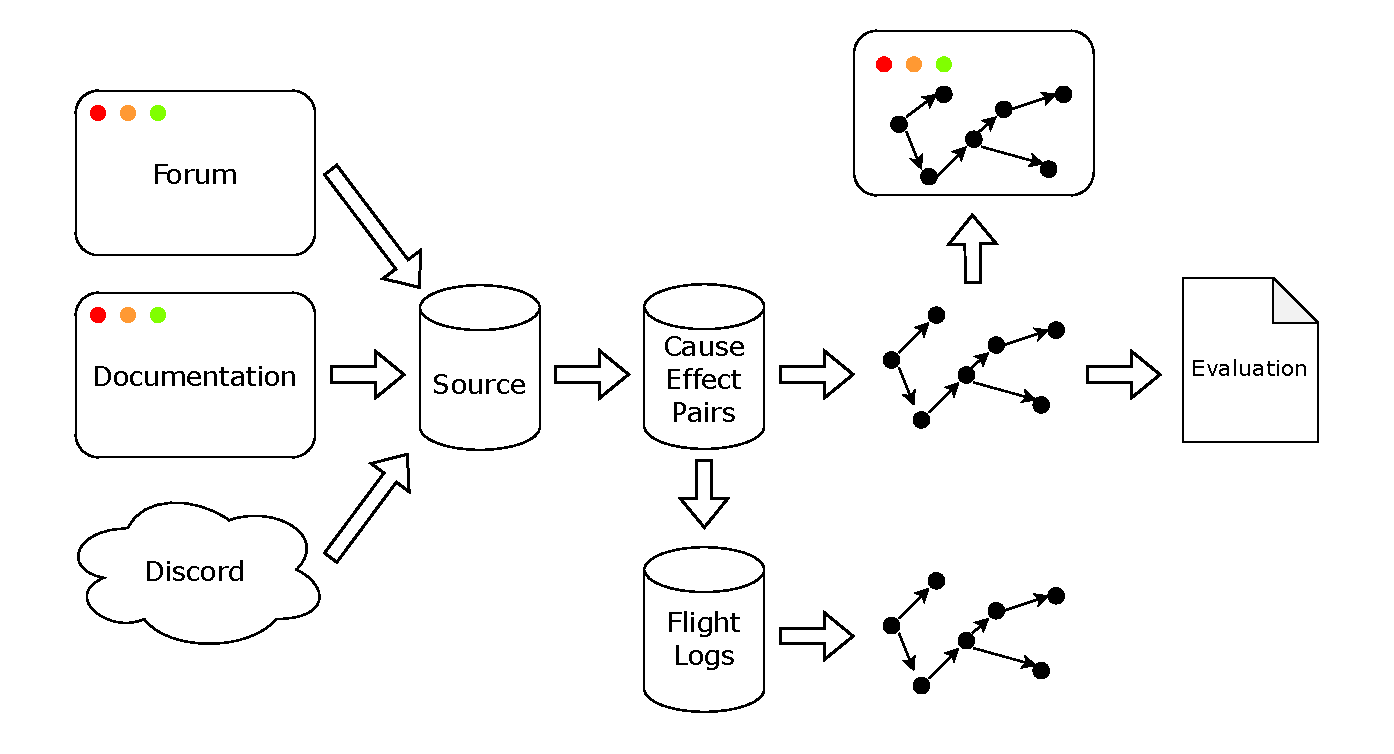
\includegraphics[width=\textwidth]{figures/pipeline_overview/pipeline_overview}
    \caption{End-to-End Pipeline Overview}\label{fig:pipeline-overview}
\end{figure}


\section{Data Collection}\label{sec:data-collection-pipeline}
The goal of this module is to provide a dataset which contains correct and cleaned sentences from domain-experts of the ArduPilot community.
We divided this module into four independent submodules to ensure an efficient and flexible scraping procedure.
The first three submodules gather raw text from the ArduPilot community channels: the discussion forum, the Discord chat, and the online documentation.
To gather the data from the different sources, we used the respective scraping techniques described in \autoref{subsec:evaluation-of-the-correct-technique}.
Next, we store the results from each module into an independent data storage, which can be filled either once when we run the pipeline from start to finish or by manually updating a specific data storage.
Finally, after we gathered the raw data from all sources, we extracted sentences from each source, gave each sentence a unique identifier, and combined the sentences into one dataset.


\section{Cause-Effect Pair Extraction}\label{sec:cause-effect-pair-extraction-pipeline}
This module takes the domain-expert sentences from the data collection module as input and outputs multiple \ac{CEP}s.
We first filter the sentences that contain explicitly mentioned causation and cache them in a dataset.
We then use this cached dataset to find \ac{CEP}s based on dependency patterns and phrase extraction techniques (see \autoref{subsec:scope-of-the-thesis}).
Finally, we store the extracted \ac{CEP}s for further processing.


\section{Causal Graph Generation}\label{sec:causal-graph-generation-pipeline}
This module consists of three submodules.
The first module takes the raw \ac{CEP}s from the previous module and transforms them into a \ac{WDCG} (see \autoref{sec:causal-graphs}).
The second module builds a \ac{WDCG} from the flight logs dataset.
We store the resulting nodes, edges, and weights for both \ac{WDCG} for further evaluation.
The last module provides an interactive tool for a \ac{WDCG} to explore the structure and trace events to root nodes back.


\section{Evaluation}\label{sec:evaluation-pipeline}
\begin{figure}
    \begin{center}
        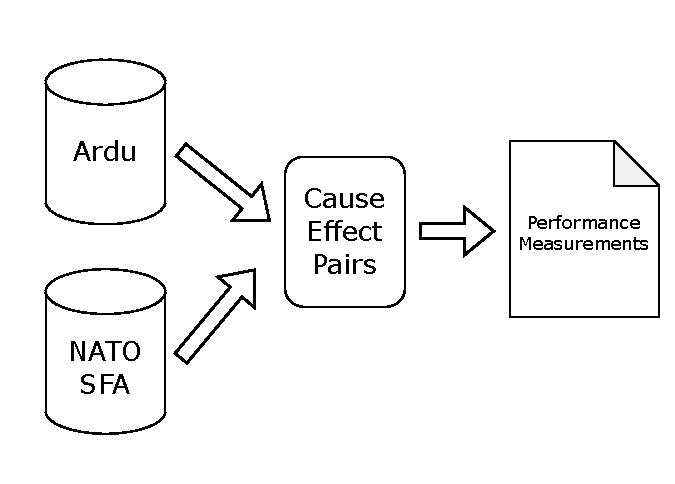
\includegraphics[scale=.7]{figures/pipeline_overview/evalutation_overview}
        \caption{Performance Measurement Overview}\label{fig:evaluation-overview}
    \end{center}
\end{figure}
The last module contains two submodules to evaluate the \ac{CEP} algorithm and the \ac{WDCG}.
The first submodule measures the performance of the \ac{CEP} extraction algorithm, which can be additionally seen in \autoref{fig:evaluation-overview}.
We use two labeled datasets to provide a domain-independent result, one from a foreign-domains and one was created from the domain-expert knowledge dataset from \autoref{sec:data-collection-pipeline}.
The second submodule analyses the \ac{WDCG} and infers the quality of the online resources.
Moreover, this submodule compares the causal graph with the flight logs graph generated in \autoref{sec:causal-graph-generation-pipeline}.

    \chapter{Data Collection}\label{ch:data-collection}

The ArduPilot software has an active community consisting of users and developers.
They have three different sources to exchange their knowledge, ask for help or get information about the system.
Unfortunately, the channels differ significantly in the availability of their content.
Therefore, we decided to provide a tailored web scraping solution for each channel.


\section{Discussion Forum}\label{sec:discussion-forum}
The discussion forum is the mainly used community channel of ArduPilot.
Users and developers can inform, discuss and ask questions about topics in the domain of \ac{UAV} systems.
This section aims to provide a methodology to build a tailored web scraper for the discussion forum.

\subsection{Structure Of The Forum}\label{subsec:structure-of-the-forum}
\begin{figure}
    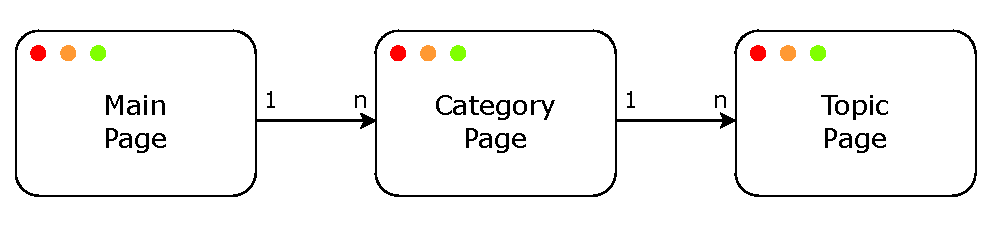
\includegraphics[width=\textwidth]{figures/data_collection/forum_structure}
    \caption{Page Structure of the Discussion Forum}\label{fig:forum-structure}
\end{figure}
First, we analyze the page structure of the forum.
In \autoref{fig:forum-structure} we can see the structure of the forum, which consists of three layers and builds a hierarchical tree.

\subsubsection{Main Page}
\begin{figure}
    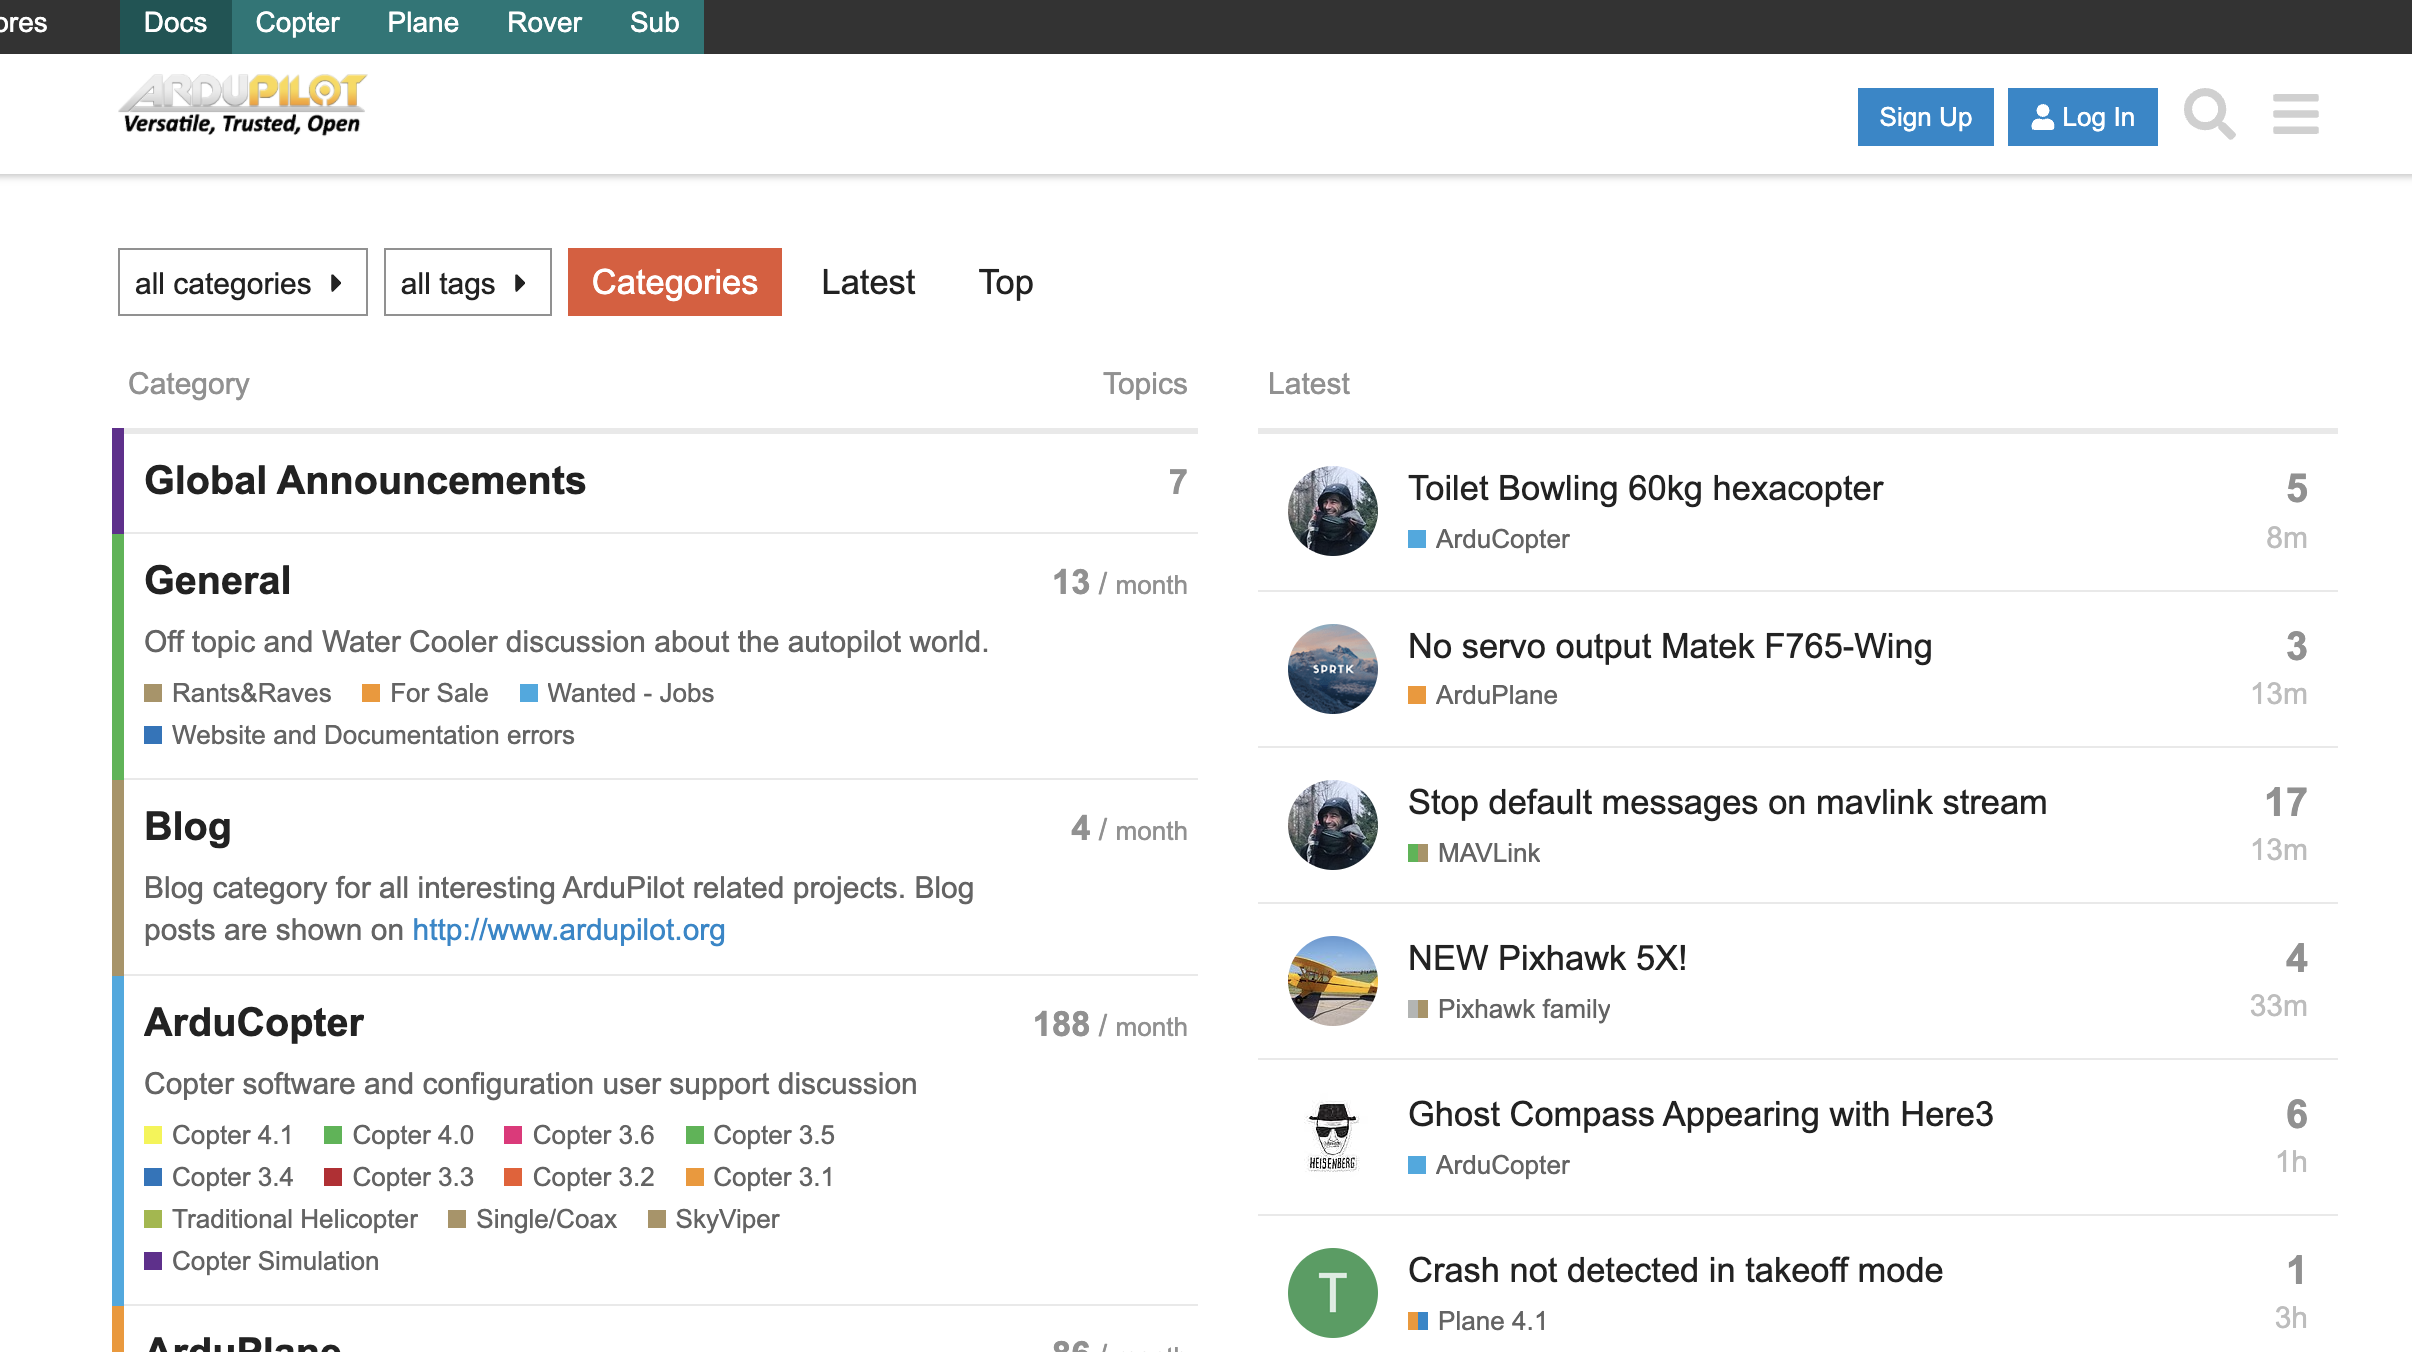
\includegraphics[width=\textwidth]{figures/data_collection/forum_main_page}
    \caption{Main Page}\label{fig:forum-main-page}
\end{figure}
The main page is the root of the structure and the starting point when joining the discussion forum.
In \autoref{fig:forum-main-page} we can see the page from the perspective of a user.
This page gives an overview of all available categories in the forum and links to the corresponding category pages.

\subsubsection{Category Page}
\begin{figure}
    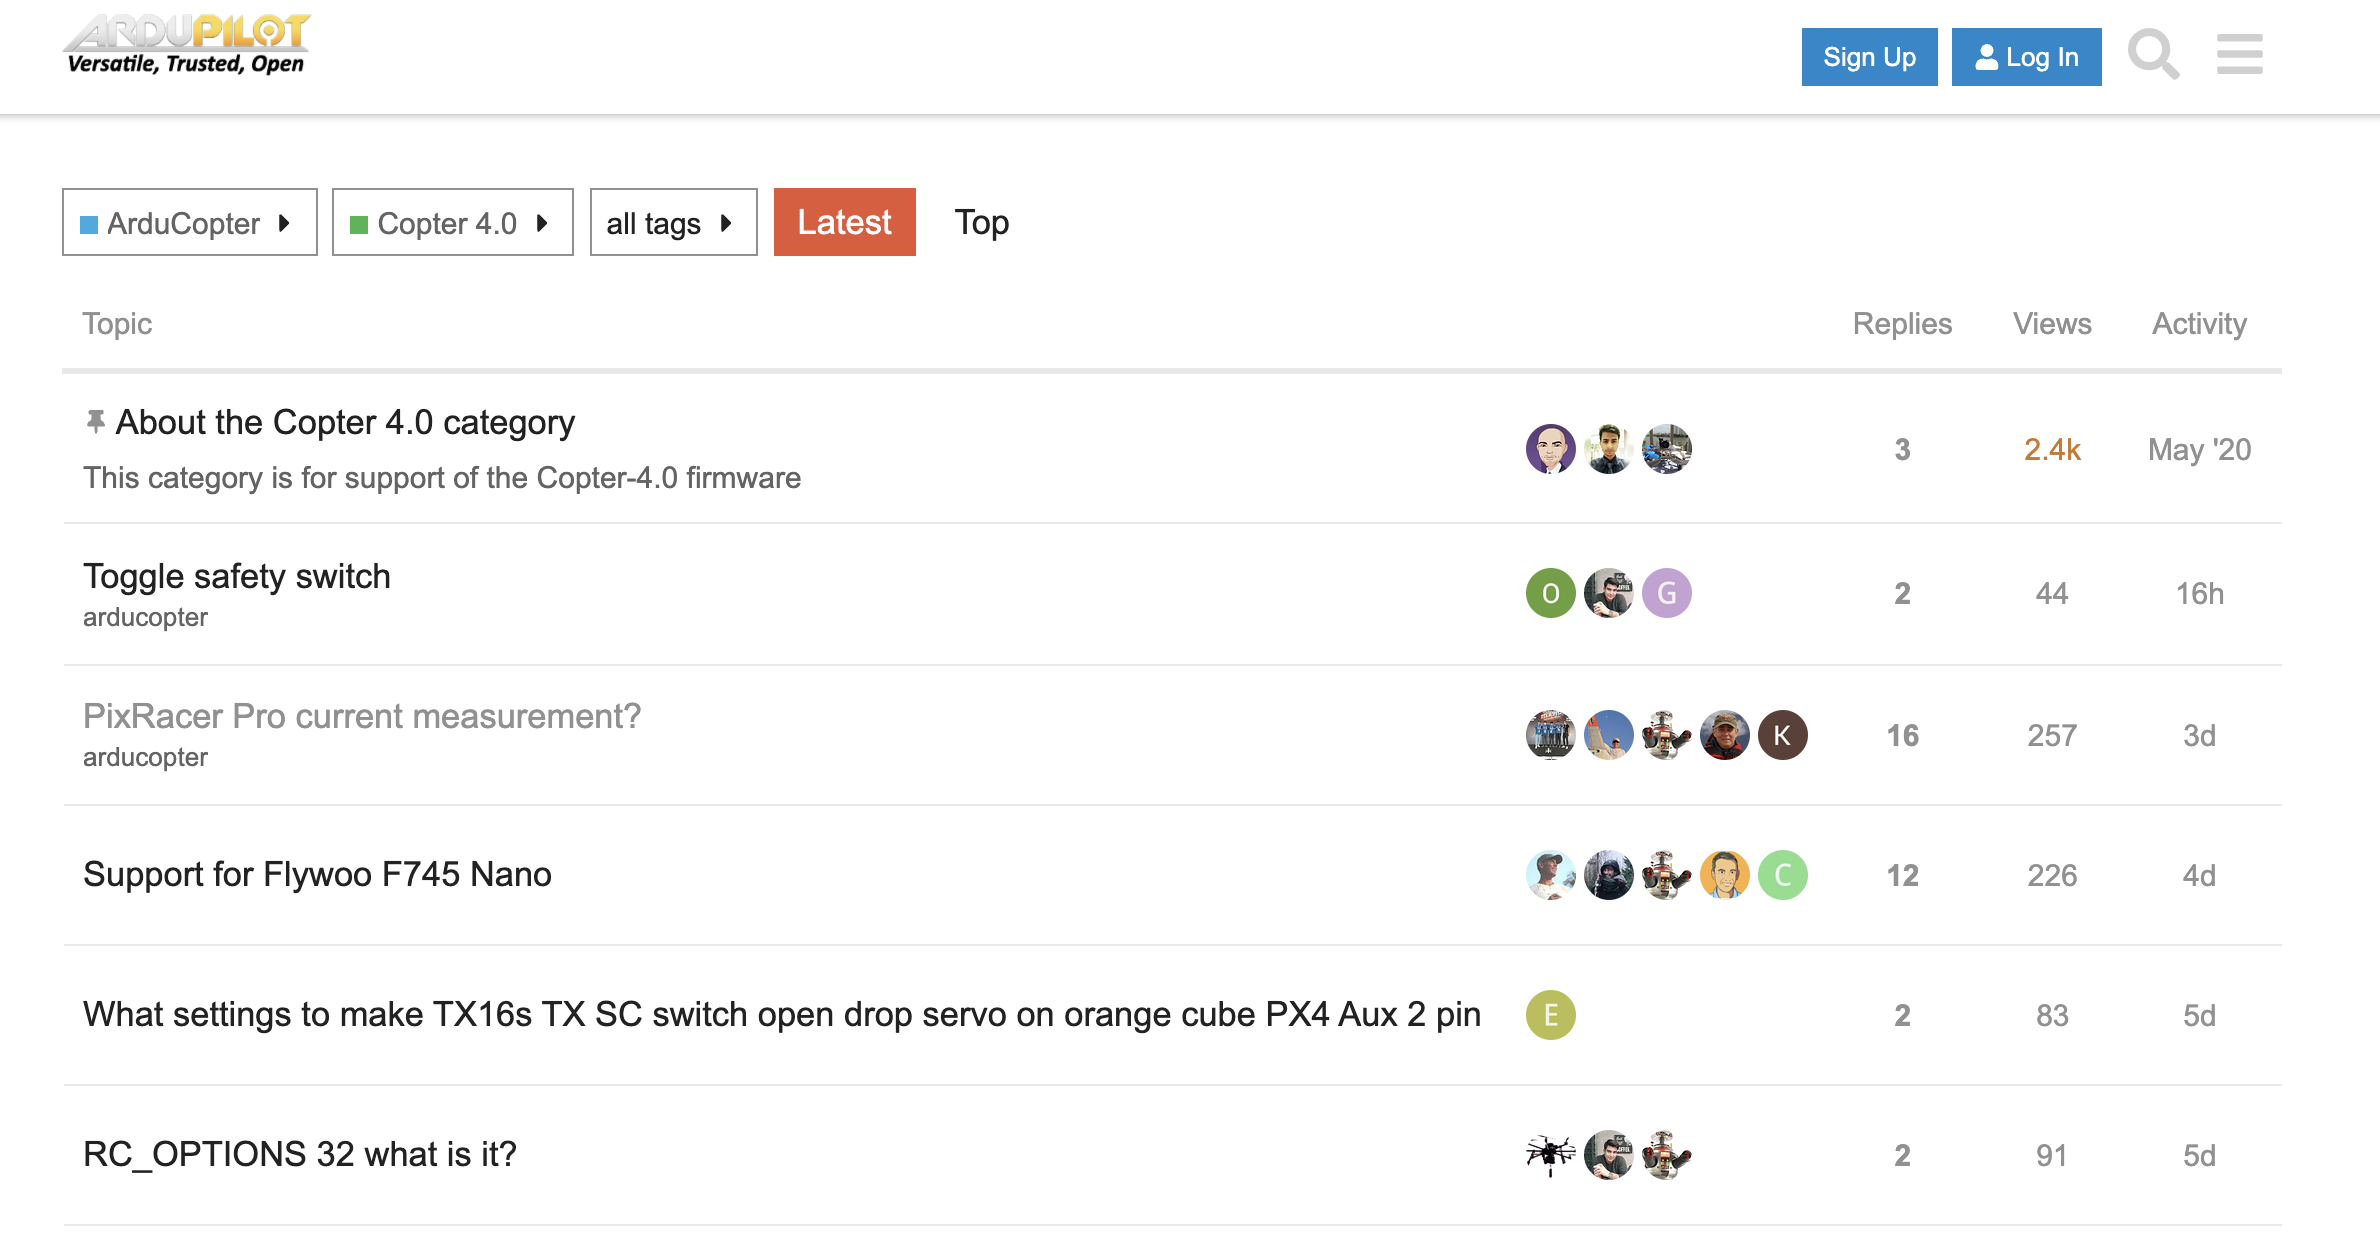
\includegraphics[width=\textwidth]{figures/data_collection/forum_category_page}
    \caption{Category Page}\label{fig:forum-category-page}
\end{figure}
The second layer is the category page, which gives an overview of all topics discussed in that category.
In \autoref{fig:forum-category-page}, we can see the category page for the root category \qq{ArduCopter} with the subcategory \qq{Copter 4.0}.
This page lists all topics linked to that category.
Additionally, different information is accessible for each topic, such as the number of users' replies, the count of the views for a topic, or the last activity.
Since such a page can have thousands of topics, the page loads new topics dynamically when a user scrolls at the bottom of the page.

\subsubsection{Topic Page}
\begin{figure}
    \begin{center}
        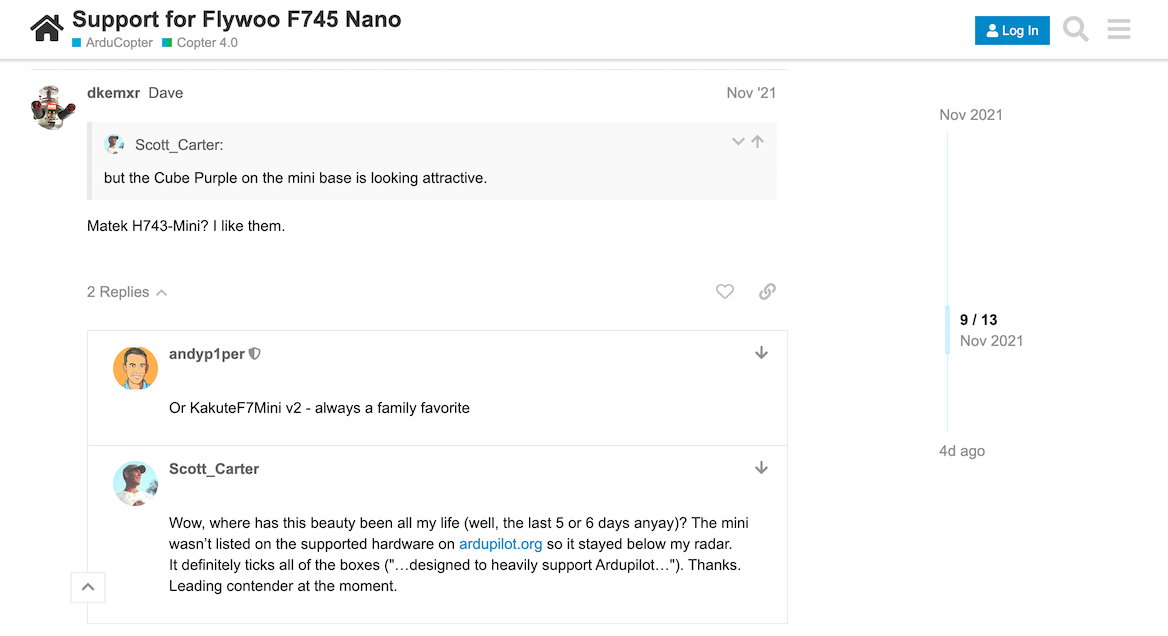
\includegraphics[width=\textwidth]{figures/data_collection/forum_topic_page}
        \caption{Topic Page}\label{fig:forum-topic-page}
    \end{center}
\end{figure}
The last layer consists of the topic page, the communication place between different users.
A user can create a new post or reply to an existing post.
For example, in \autoref{fig:forum-topic-page}, we can see the topic page for \qq{Support for Flywoo F745 Nano}.
Like the category page, it loads the posts dynamically when the user scrolls to the bottom.
However, the page only stores 25 posts per time in the \ac{HTML}.
Thus, if the user scrolls and loads new posts, previous loaded posts will unload.
Furthermore, the replies on the posts are only accessible by clicking on a \qq{Replies} button.
The knowledge contains in these communications.
Thus, we want to gather the textual context for all posts and their replies.
Having a direct way to access a specific post without dealing with the topic page's dynamic load and unload behavior would benefit an efficient web scraping solution.
Fortunately, there is a unique \ac{URL} representation for each post.
For example, \url{https://discuss.arupilot.org/t/support-foru-flywoo-f745-nano/77952/3} is the \ac{URL} for the third post for the topic \qq{Support for Flywoo F745 Nano}.
We can build such a \ac{URL} by knowing the position of the post on the topic page and the \ac{URL} of the topic page by ourselves.
We receive the topic page \ac{URL} from the category page and the category page \ac{URL} from the root page.
Thus, to build the \ac{URL} for a specific post, we have to go through all layers on the forum.

\subsection{Web Scraper System Overview}\label{subsec:building-the-web-scraper}
\begin{figure}
    \begin{center}
        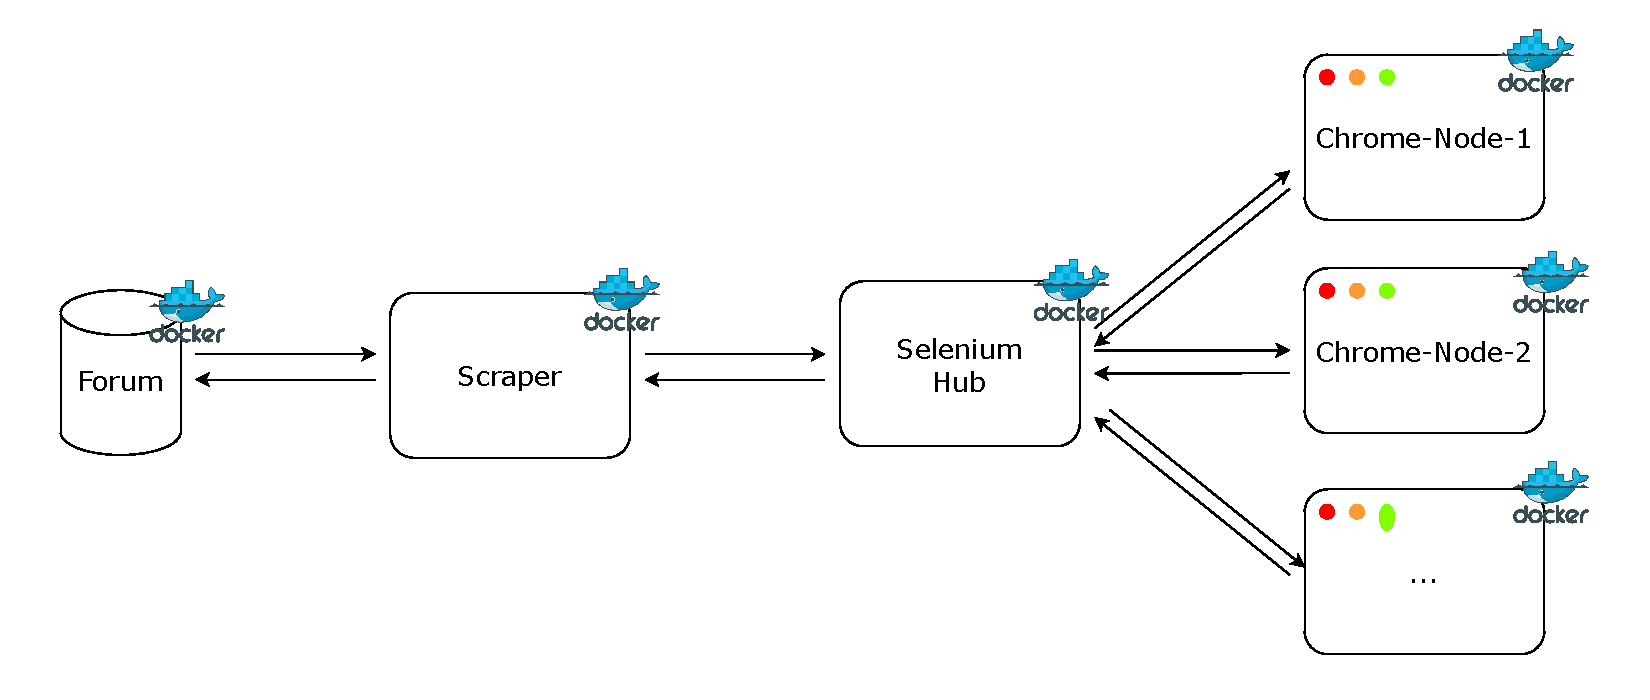
\includegraphics[width=\textwidth]{figures/data_collection/forum_scraper_architecture}
        \caption{Forum Web Scraper Architecture}\label{fig:forum-scraper-architecture}
        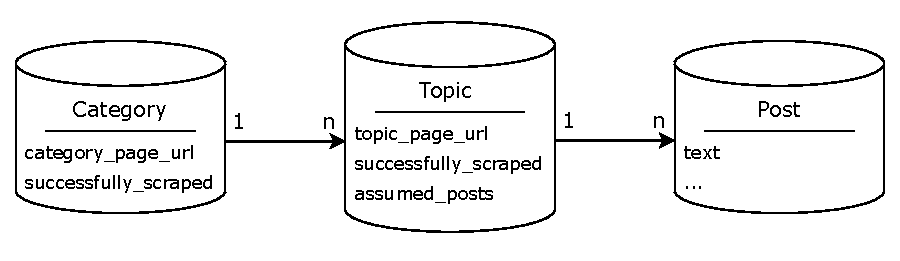
\includegraphics[scale=0.7]{figures/data_collection/forum_data_architecture}
        \caption{Forum Database Tables}\label{fig:forum-data-architecture}
    \end{center}
\end{figure}

This section provides an efficient, scalable, and robust way to access all posts and replies for these high dynamic webpages.
In \autoref{fig:forum-scraper-architecture} we can see the architecture of such a web scraper, consisting of at least four isolated docker\footnote{\url{https://www.docker.com/}} containers: a database, a web scraper, a hub, and multiple nodes, where the last two containers build a Selenium Grid\footnote{\url{https://github.com/SeleniumHQ/docker-selenium}}.
The first container hosts a PostgreSQL\footnote{\url{https://www.postgresql.org/}} database.
In \autoref{fig:forum-data-architecture} we can see the tables of the database, which are closely related to the page structure.
In the database, we store the scraped post contents and the \ac{URL}s for the different pages, information about the scraping status, and meta-information about the pages.
We use SQLAlchemy\footnote{\url{https://www.sqlalchemy.org/}}  to define our table schema and communicate with the PostgreSQL database.
The second container runs the web scraper.
The core of the scraper is the Selenium library which defines the logic for scraping new URLs or gathering content based on manually defined XPaths and CSS selectors.
We choose Selenium because it automates web browser interaction by communicating to the Selenium Grid.
We chose a Selenium Grid setup over a single web driver setup because it allows us to handle multiple web drivers parallel.
Furthermore, in combination with the Selenium Grid, Selenium allows us efficiently scroll down a page or click on a button, which is needed to access all topics on the category page or click on the \qq{Replies} button.

\subsection{Web Scraping Routine}\label{subsec:web-scraping-routine}
A docker-compose command triggers our web scraping routine after the Selenium Grid, and the database container is started.
We follow the layout structure of the discussion forum to gather all post \ac{URL}s.
First, we scrape the category page \ac{URL}s from the main page, which can be done by following the XPath to the corresponding \ac{HTML} elements.
Then we scrape for each category page all topic page URLs. Next, we use Selenium and the interaction with the web browser to scroll to the bottom of the category page to load all topics.
We store the topic page \ac{URL}s and the number of replies in the database.
The last step is to scrape all the posts by building unique post \ac{URL}s from the topic page \ac{URL} and the rank of the post on the page.
Using the number of replies, we know the upper bound of the possible ranks of the posts on a page.
Therefore, we can build all unique post \ac{URL}s by a simple loop over the number of replies, where the loop index is similar to the rank.
There is one significant speed improvement by using the dynamic behavior of the topic page, where 25 posts are loaded per request.
Thus, we can significantly speed up the scraping by generating each twenty-fifth \ac{URL} and scraping the content for the other posts at once.
Unfortunately, Selenium Grid can have a timeout exception after several hours of scraping, triggering a WebDriverException in Selenium.
To handle these errors, we wrap the previous scraping routine in a try-catch block which triggers a docker-compose restart when an exception occurs.
Thus, the scraping script will start from the beginning.
To continue the old progress, we store an additional attribute $scraped\_successfully$ to the category and topic table, which allows us to skip the pages marked as $scraped\_successfully$.
The previous steps allow us to scrape the dynamic discussion forum efficiently and robustly.


\section{Documentation}\label{sec:documentation}

\subsection{Structure Of The Documentation}\label{subsec:structure-of-the-documentation}
\begin{figure}
    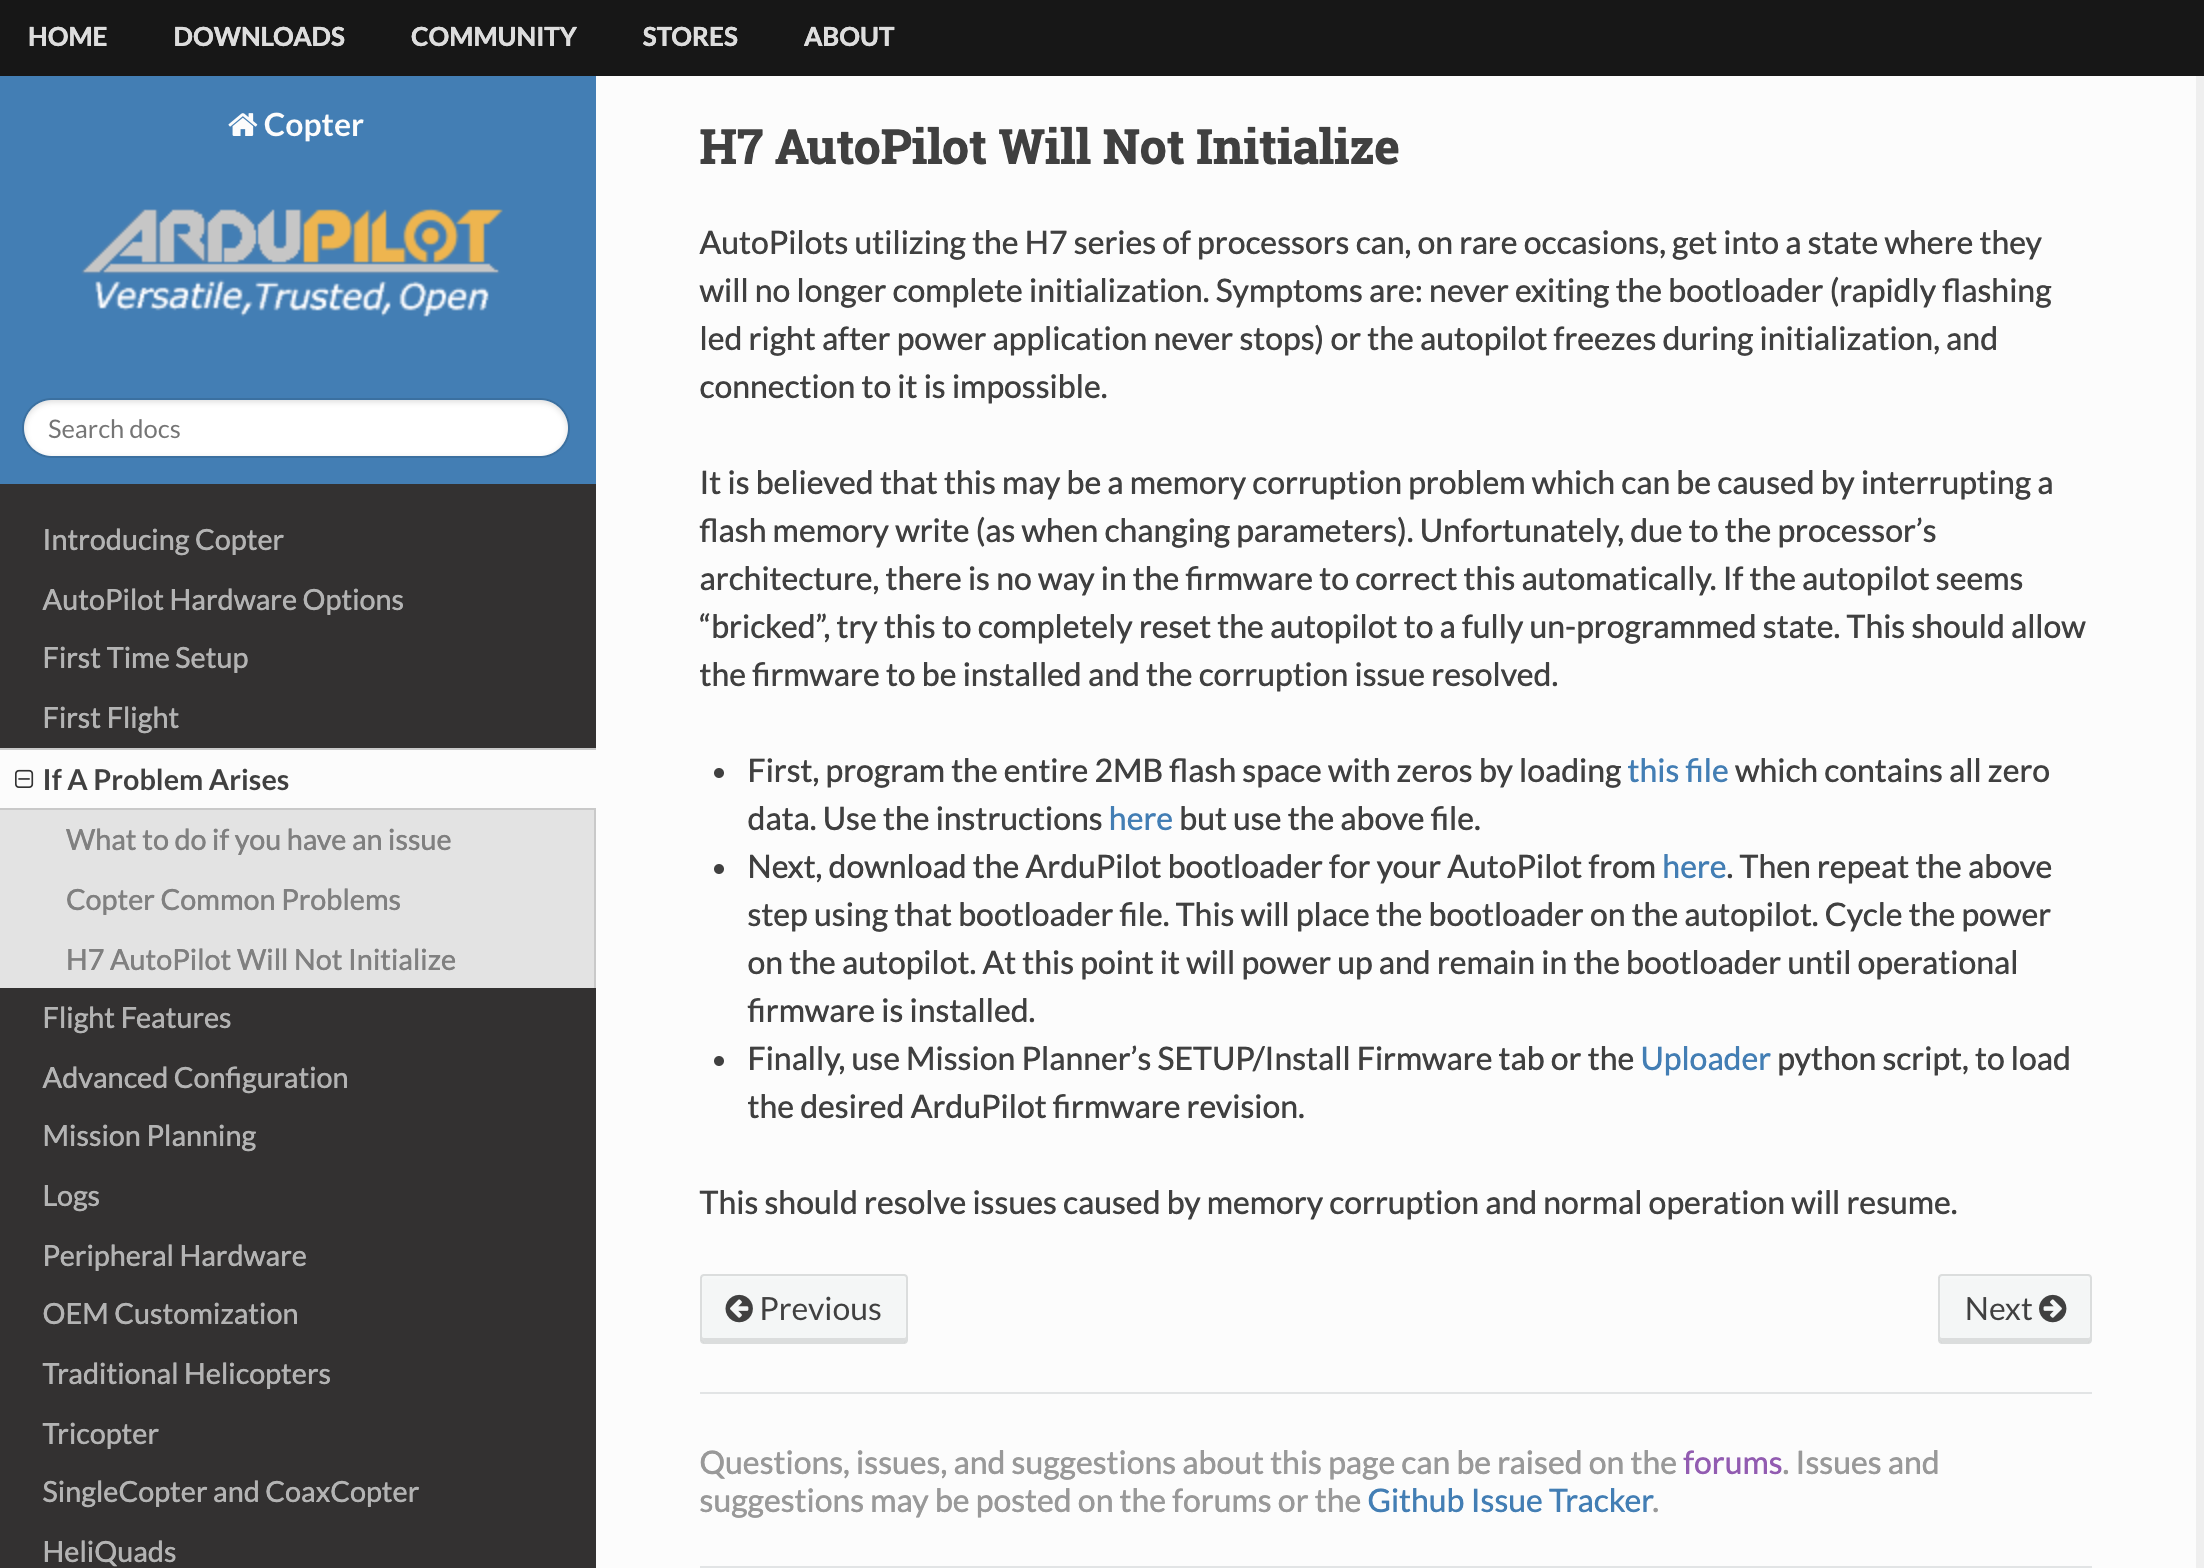
\includegraphics[width=\textwidth]{figures/data_collection/documentation_full_page}
    \caption{Documentation Page}\label{fig:documentation-full-page}
\end{figure}

Ardupilot provides online documentation about their software, which their developers maintain.
We also want to use this source because it is high quality and covers the ArduPilot system.
It also differs from the discussion forum and the discord chat in that the content is more structured with less noise which can be seen in \autoref{fig:documentation-full-page}.
The documentation consists of three main sections.
The first section is the navigation sidebar on the left, which gives an overview of all documentation topics.
The second section provides the content of a specific documentation page, which is loaded statically and therefore accessible without interacting with the page.
The last part consists of two buttons, \qq{Next} and \qq{Previous}, which allow navigating between the pages.
The documentation pages are fully connected, allowing it to access all documentation pages by only clicking on the \qq{Next} button when starting at the beginning.

\subsection{Scraping Strategy With Scrapy}\label{subsec:scrapy}
We decided to use Scrapy, a web crawling and scraping framework, to gather the structured data from the documentation page.
Scrapy uses spiders, which define how a specific site will be scraped, including how to perform the crawl and how to extract the data.
The spider acts in a cycle with the following steps:
\begin{enumerate}
    \item Start the scraping with an initial request to crawl the first \ac{URL} and define a callback function that handles the response.
    \item The callback function parses the page content using Selectors like XPath and combines the information into Scrapy items.
    We can also define a new request at the end of the callback function to build that cycle and repeat at 1).
    \item The items returned from the spider will be persisted in a database.
\end{enumerate}
We build a spider that starts at the root page of the documentation.
Next, we create a callback function that extracts the documentation page's textual content, which extracts the \ac{URL} from the \qq{Next} button.
Finally, we build the cycle by sending a new request with that \ac{URL} until we are at the end of the documentation.
Thus, we built a simple yet efficient and easily maintainable web scraper for online documentation.


\section{Discord}\label{sec:discord-webscraping}
The Discord platform is the main communication platform for the developers of the ArduPilot system.
There, the developers chat in different channels mainly about technical details and problems with the software.
Fortunate Discord provides a developer API\footnote{\url{https://discord.com/developers/docs/reference}} to scrape chat messages from channels directly.
We need to provide an authentication token in the request header to access the \ac{API}.
A simple GET request uses \url{https://discord.com/api/v9/channels/[channel_id]} as a \ac{URL} to access messages for a specific channel.
However, the Discord \ac{API} limits the number of response messages and returns only the latest messages.
Fortunate, we can specify path parameters to the GET request which looks like \url{https://discord.com/api/v9/channels/[channel_id]/messages?limit=[limit]&before=[before_id]}.
For the scope of our \ac{API} scraper, we only need to consider the $limit$ and the $before$ path parameter.
The $limit$ path parameter specifies the number of messages returned on a single request.
The default is 50, but it can be extended to 100 at most.
Furthermore, we can get older messages by setting the $before$ path parameter to some $messages\_id$.
Thus, we can build an efficient \ac{API} scraper that scrapes the messages from the channel, which consists of three parts:
\begin{enumerate}
    \item Send the initial request and specify the $channel\_id$ and the $limit$ path set to max.
    \item Extract the content of the message from the response and store the result in a database.
    \item If the response size is the same as the specified limit size, there are more messages in the chat.
    Thus, we extract the $message\_id$ from the last response item
    Finally, we send another request which specifies the $before$ parameter with the $message\_id$.
    We then continue at 2).
\end{enumerate}


\section{Merging And Cleaning}\label{sec:merging-and-cleaning}
The previous subsection described the different web scarping strategies for the ArduPilot channels.
Each of these scrapers produced a dataset containing raw textual information.
Unfortunately, the characteristics of the sources lead to a \qq{dirty} data source.
There are several reasons for the poor data quality in chat-based environments, which are closely connected to the user's behavior in online communication''
\begin{itemize}
    \item One logical sentence could be split into different paragraphs, which happens when a user places images inside a sentence or starts a new line accidentally.
    \item Extensive usage of a short text that includes no information like \qq{Hi}, \qq{no} or \qq{that's true}.
    \item The text contains special characters, e.g., smileys or links to other chat messages, users, or channels represented with their ids like \qq{@483512342}.
\end{itemize}

\subsection{Cleaning And Extracting Sentences}\label{subsec:cleaning-and-extracting-sentences}
We provide a pipeline that extracts correct, formatted, and cleaned sentences from raw textual data, implementing four steps:
\begin{enumerate}
    \item Preprocessing with regular expression: In the first step, we convert the raw text into an ASCII representation of the text and substitute the whitespace characters like $\setminus n$, $\setminus t$ or a sequence of whitespaces with a simple whitespace character.
    Additionally, the domain requires specific regular expression substitutions to handle $user\_id$s or links to other \ac{URL}s, which do not provide information.
    We could either drop such an occurrence or replace it with something meaningful.
    We decided to replace it with a generic representation like \qq{User} or \qq{URL} to maintain the structure of the sentence.
    \item Sentence segmentation: The following step was to extract the sentences from the pre-processed text.
    We could create a bunch of regular expression rules to find the boundaries of a sentence.
    However, the sentences could be represented ambiguously, and the users could format or mark the start and end of a sentence that is not reflected in our patterns.
    Therefore, we decided to use the spaCy\footnote{\url{https://spacy.io/}} library to detect sentence boundaries based on a pre-trained \ac{NLP} model (see \autoref{ch:cause-effect-extraction}).
    These extracted sentences do not necessarily have to end with punctuation or start with an uppercase.
    Therefore, we substituted the first character with an uppercase and added punctuation.
    \item Grammar checker: The sentence segmentation also extracts short sentences without information such as \qq{Hi!} or \qq{That is true}.
    We do not want to include such sentences in the resulting dataset.
    Thus, we decided to drop sentences that do not meet the standards for a complete sentence, which means that we drop sentences without a verb, an object, or a subject.
    \item Remove duplicate mentions: It is common to reference other messages or posts in a chat-based environment.
    In \autoref{fig:forum-topic-page} we can see an example of such a reference.
    When a user references another post, the content of the reference will be injected into the user's post.
    Thus, we have duplicate sentences that are from the same source.
    Hence, we decided to drop such sentences.
\end{enumerate}

\subsection{Merging Into One Source}\label{subsec:merging-to-one-source}
The last step of the data collection pipeline is to combine the extracted sentences from the different sources into one source.
We decided to combine everything into a single CSV file because it makes it easier to explore the dataset and share it with other researchers.
The dataset consists of three columns:
\begin{itemize}
    \item id - integer: A unique identifier for a sentence which is especially useful when you want to backtrack the sentence at the different pipeline stages.
    \item sentence - string: A sentence that is mentioned by a domain expert from the Ardupilot community.
    \item source - string: A categorical variable that is either \qq{forum}, \qq{docs} or \qq{chat}, which indicates the source of the sentence.
\end{itemize}
This dataset represents the domain-expert knowledge about the users and developers of the Ardupilot system.

    \chapter{Cause-Effect Pair Extraction}\label{ch:cause-effect-extraction}
This chapter will provide a methodology to extract multiple \ac{CEP}s from a sentence, by using dependency patterns and a novel phrase extraction algorithm.


\section{Natural Language Processing}\label{sec:natural-language-processing}

\begin{figure}
    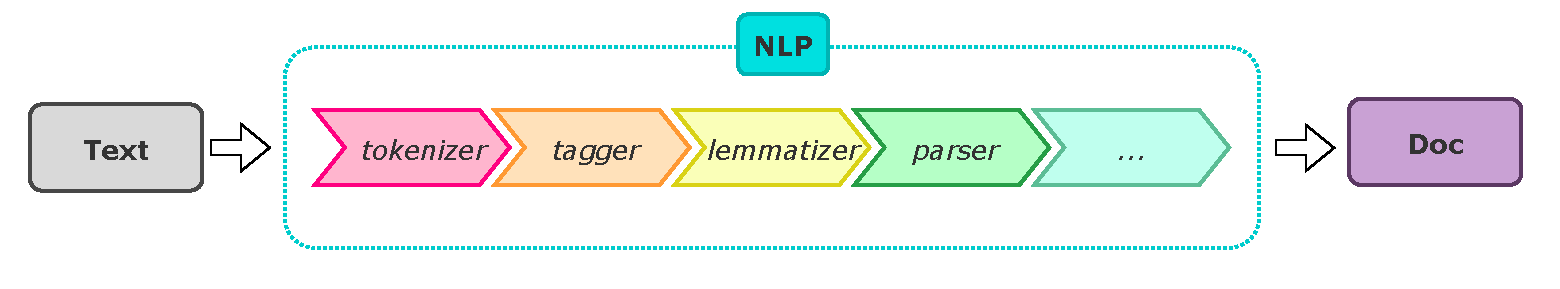
\includegraphics[width=\textwidth]{figures/cause_effect_extraction/spacy_pipeline}
    \caption{NLP Pipeline}\label{fig:spacy-pipeline}
\end{figure}

The first step of our extraction algorithm takes a text and pass it through a \ac{NLP} pipeline.
Fortunate, several NLP libraries such as spaCy utilizes such pipelines with pretrained models to add linguistic features to the text.
In \autoref{fig:spacy-pipeline} we can see the simplified pipeline for the \qq{en\_core\_web\_lg} model\footnote{\url{https://spacy.io/models/en\#en_core_web_lg}} from the spaCy library.
Such pipeline can contain several of different layers and implementation details.
Our approach to \ac{CEP}s is based on dependency patterns.
Thus, the pipeline needs to have a tokenizer, tagger, lemmatizer and parser.

\subsection{Tokenizer}\label{subsec:tokenizer}
The tokenizer splits the text into meaningful segments, called tokens.
These tokens could be words, punctuations, combinations of abbreviations or other segments.
For example the word \qq{don’t} should be divided into two tokens whereas a word like \qq{v1.0} should be remains at one token.
There are several implementations of such tokenizer, we used the built-in tokenizer from spaCy which first splits the raw text based on whitespace characters.
Next, the algorithm loops over the substrings and tries to split them into more granular tokens based on different rules, such as prefix, suffix, punctuation and more.
The tokens are the foundation for the following pipeline.

\subsection{Tagger}\label{subsec:part-of-speech-tagging}
The first label added to the tokens is the \ac{POS}\footnote{\url{https://universaldependencies.org/u/pos/}} label.
This tag can be divided into three groups.
The first group contains open class words such as adjective (ADJ), noun (NOUN), proper noun (PROPN) or verb (VERB).
The second group are closed class words such as determiner (DET) or pronoun (PRON).
The last group contains the other tags such as punctuation (PUNCT).

\subsection{Lemmatizer}\label{subsec:lemmatizer}
The next component is the lemmatizer which groups different inflected forms into a single word.
For example, the words \qq{works}, \qq{worked} or \qq{working} would have all the same lemma \qq{work}.
Another advantage of a lemmatizer is that it also does the morphological analysis of words.
Thus, it detects \qq{good} as a lemma for the word \qq{better}, which is especially useful if we want to compare different tokens with each other.

\subsection{Parser}\label{subsec:dependency}
The last step is the dependency parser which adds the \ac{DEP}\footnote{\url{https://downloads.cs.stanford.edu/nlp/software/dependencies_manual.pdf}} tag to a token.
This preprocessing step connects different tokens with each other, which allows us to represent the sentence in a dependency tree and apply dependency patterns to the sentence.
For example, the \qq{nsubj} tag defines a syntactic subject of a clause.
In \autoref{sec:dependency-matching} we will see the needed \ac{DEP} tags to define the dependency patterns.


\section{Dependency Matching Patterns}\label{sec:dependency-matching}
After pre-processing the sentence by passing it through an \ac{NLP} pipeline, we want to find the root tokens for the \ac{CEP}.
In \cite{doan2019extracting, sorgente2013automatic}, the authors provided dependency patterns to identify \ac{CEP}s with a single word.
For example, if we look at the sentence \qq{A GPS fault causes a crash.}, these patterns find \qq{fault} => \qq{crash} as a \ac{CEP}.
We implement these patterns using the DependencyMatcher\footnote{\url{https://spacy.io/usage/rule-based-matching\#dependencymatcher}} from spaCy, which utilizes Semgrex operators on a dependency tree to match patterns.
In \autoref{fig:pattern-simple}, \autoref{fig:pattern-phrasal} and \autoref{fig:pattern-passive} on the left side are example patterns that can be implemented with the DependencyMatcher.
These patterns consist of nodes that are connected over Semgrex operators.
For example, the node \qq{A} and \qq{B} defines a pattern with the \qq{>} Semgrex operator, which looks like \qq{A > B}.
The pattern matches when in the dependency tree the node \qq{A}, the immediate head of \qq{B} is.
We can add attributes to the nodes that define additional rules that the node needs to fulfill.
For example, we could specify a lemma representation of a word that we want to match or a specific \ac{POS} tag that needs to be fulfilled.
Furthermore, these patterns have one anchor node, which is equivalent to a root in a tree, which is the starting point for the DependencyMatcher.
We use this anchor node to find explicit causal mentions based on a list of low ambiguity and high frequency causation verbs provided by \cite{girju2002text}.
The most common causal identifiers are \qq{cause}, \qq{lead}, \qq{generate} and \qq{trigger}.
Furthermore, we used a verb list consisting of 26\footnote{cause, generate, trigger, induce, produce, effect, provoke, arouse, elicit, lead, derive, associate, relate, link, stem, iginate, result, entail, commence, spark, evoke, implicate, activate, actuate, kindle, stimulate, unleash, effectuate} verbs.
We are now building our anchor node by specifying the lemmatized verb list as additional rule.
Thus, we are able to find different variations of the verb \qq{cause} like \qq{causes} or \qq{caused}.
Based on this anchor node we specify outgoing dependency nodes which are connected to the root token for the cause and the effect in the \ac{CEP}.

\subsection{Simple Causative Verbs}\label{subsec:simple-causative-verbs-pattern}
\begin{figure}
    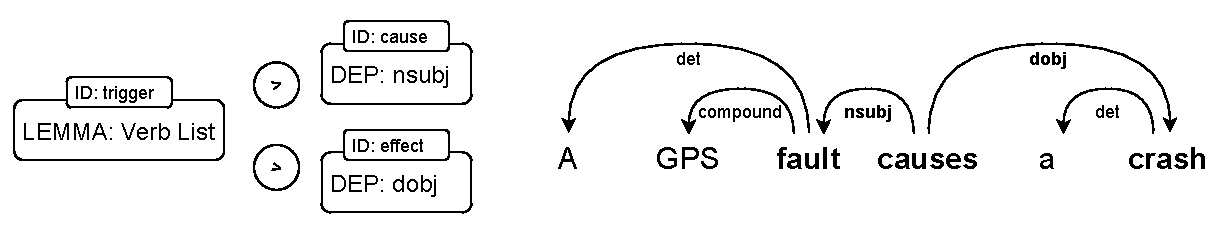
\includegraphics[width=\textwidth]{figures/cause_effect_extraction/simple_pattern}
    \caption{Simple Causative Verbs Pattern}\label{fig:pattern-simple}
\end{figure}
The pattern has as anchor having the meaning of a simple \qq{causal action} such as \qq{cause}, \qq{generate}, or \qq{trigger}.
In this pattern, the cause is the subject of that simple verb, and the effect is the verb's object, which can be seen on the left side of the \autoref{fig:pattern-simple}.
Furthermore, we can see on the right side of \autoref{fig:pattern-simple} an example sentence that is covered by this pattern.
By comparing the sentence with the pattern, we see how dependency matching works.
First, the causal anchor is selected like \qq{causes} which is then be used to find the other tokens that match with the described pattern like \qq{fault} and \qq{crash}
The DependencyMatcher then provides the tokens that match with the pattern, thus  \qq{causes} \qq{fault} and \qq{crash}.
Finally, we specified an ID for each node in the pattern to distinguish the tokens.

\subsection{Phrasal Verbs}\label{subsec:phrasal-verbs-pattern}
\begin{figure}
    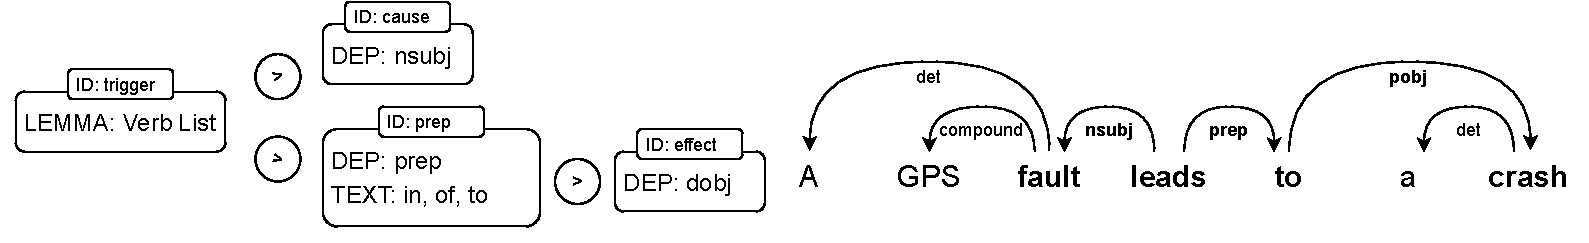
\includegraphics[width=\textwidth]{figures/cause_effect_extraction/phrasal_pattern}
    \caption{Phrasal Verbs Pattern}\label{fig:pattern-phrasal}
\end{figure}
This pattern uses a phrase consisting of a causal verb followed by a preposition like \qq{in}, \qq{of} or \qq{to,} e.g. \qq{lead to} to identify an explicit causal mention.
We then follow the \qq{nsubj} \ac{DEP} from the verb to find the cause and the \qq{pobj} \ac{DEP} from the preposition to find the effect.
In \autoref{fig:pattern-phrasal} we can see the resulting pattern as well as an example sentence that matches with the pattern.

\subsection{Passive Causative Verbs}\label{subsec:passive-causative-verbs-pattern}
\begin{figure}
    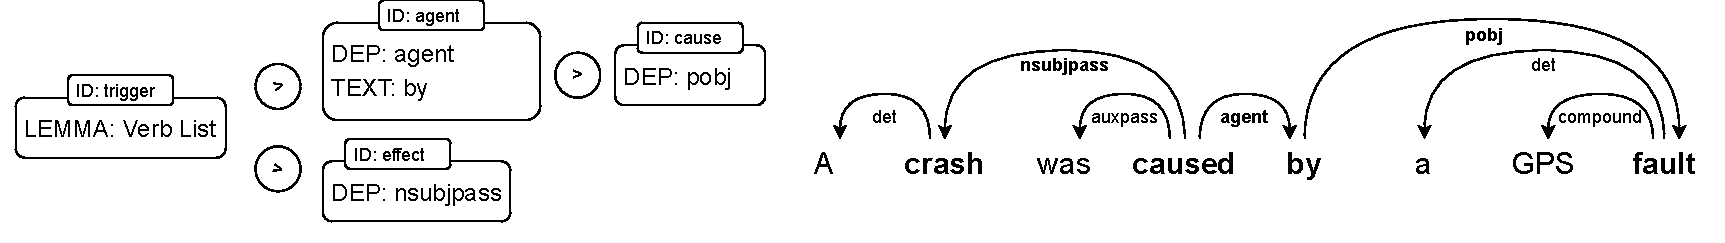
\includegraphics[width=\textwidth]{figures/cause_effect_extraction/passive_pattern}
    \caption{Passive Causative Verbs Pattern}\label{fig:pattern-passive}
\end{figure}
The last pattern we defined is for passive formulations of a sentence.
For example, a user could formulate the same sentence passive like \qq{A crash was caused by a GPS fault} which can be seen in \autoref{fig:pattern-passive}.
Therefore, the pattern uses the preposition \qq{by} that is linked to a verb from the verb list with an \qq{agent} relation.
The \qq{agent} relation is the complement of a passive verb that does the action.
Thus, the cause root is linked with the \qq{pobj} relation to the \qq{by} agent, where \qq{pobj} is the object of a preposition.
The effect is linked with the \qq{nsubjpass} to the causal verb, where \qq{nsubjpass} is a passive nominal subject which is the syntactic subject of a passive clause.
The resulting pattern can be seen in \autoref{fig:pattern-passive}.

\section{Phrase Extraction}\label{sec:phrase-extraction}
With the dependency matching patterns, we are able to identify the root token of the cause and effect.
However, in a sentence from \autoref{fig:pattern-simple} , the resulting \ac{CEP} would be \qq{fault} => \qq{crash} which omits information.
We want to extract phrases that consist of multiple tokens.
Thus, the desired \ac{CEP} looks like \qq{GPS fault} => \qq{crash}.
Furthermore, our current extraction is limited, with only a single CEP extraction on a causal identifier.
We also want to provide a methodology that extracts multiple CEPs that are connected with conjunctions such as \qq{and}, \qq{or}.
In the following, we do not differ between \qq{and}, \qq{or} although in logical rules they have a different meaning.
We decided to do that because in NLP, especially in communication, conjunctions and disjunctions are not applied in a logical way.
Therefore, if a user would say, \qq{A GPS fault, defect motor or empty battery causes a crash} we would extract three \ac{CEP}s \qq{GPS fault} => \qq{crash}, \qq{empty battery} => \qq{crash} and \qq{defect motor} => \qq{crash}.
In the previous example, we saw that the cause from the pairs had no intersecting part and was completely divided by the conjunction.
However, in the sentence \qq{An empty and defect battery causes a crash} the conjunction is between \qq{empty} and \qq{defect} and describes the root token battery.
There are two possible solutions to solve such conjunctions.
The first one is to ignore such conjunctions and extract the whole phrase as one.
We would extract \qq{empty and defect battery} as one phrase.
The second approach is to extract two phrases, \qq{empty battery} and \qq{defect battery}.
We decided to follow the second approach because we want to extract the atomic representation of a \ac{CEP}, which is more suitable to build a causal graph.
We, therefore, want to present a recursive algorithm that is capable of extracting multiple phrases based on a single root token.

\subsection{Algorithm}\label{subsec:algorithm}

\begin{algorithm}
    \algblockdefx{ForEach}{EndForEach}[1]{\textbf{for each} #1 \textbf{then}}{\textbf{end for each}}
    \caption{Phrase Extraction Algorithm}\label{alg:phrase-pseudocode}
    \begin{algorithmic}[1]
        \Require $token$ with dependency links
        \Function{ExtractPhrases}{$token$}

            \If{$token.children$ is empty}
                \State \textbf{return} $[[token]]$
            \EndIf


            \State $phrases \gets []$

            \If{$HasChildrenWithPhraseDependency(token)$}
                \State $children\_phrases \gets []$
                \ForEach{$child \in ChildrenWithPhraseDependency(token)$}
                \State $child\_phrases \gets ExtractPhrases(child)$
                \State $children\_phrases \gets Insert(children\_phrases, child\_phrases)$
                \EndForEach
                \State $combined\_children\_phrases \gets ReduceWithProduct(children\_phrases)$
                \State $token\_phrases \gets InsertAndSortTokenIntoChildrenPhrases(combined\_children\_phrases)$
                \State $phrases  \gets Extend(phrases, token\_phrases)$
            \Else
                \State $phrases  \gets Extend(phrases, [[token]])$
            \EndIf

            \ForEach{$child \in ChildrenWithConjDependency(token)$}
            \State $conj\_phrases \gets ExtractPhrases(child)$
            \State $phrases  \gets Extend(phrases, conj\_phrases)$
            \EndForEach

            \State \textbf{return} $phrases$
        \EndFunction
    \end{algorithmic}
\end{algorithm}

\begin{figure}
    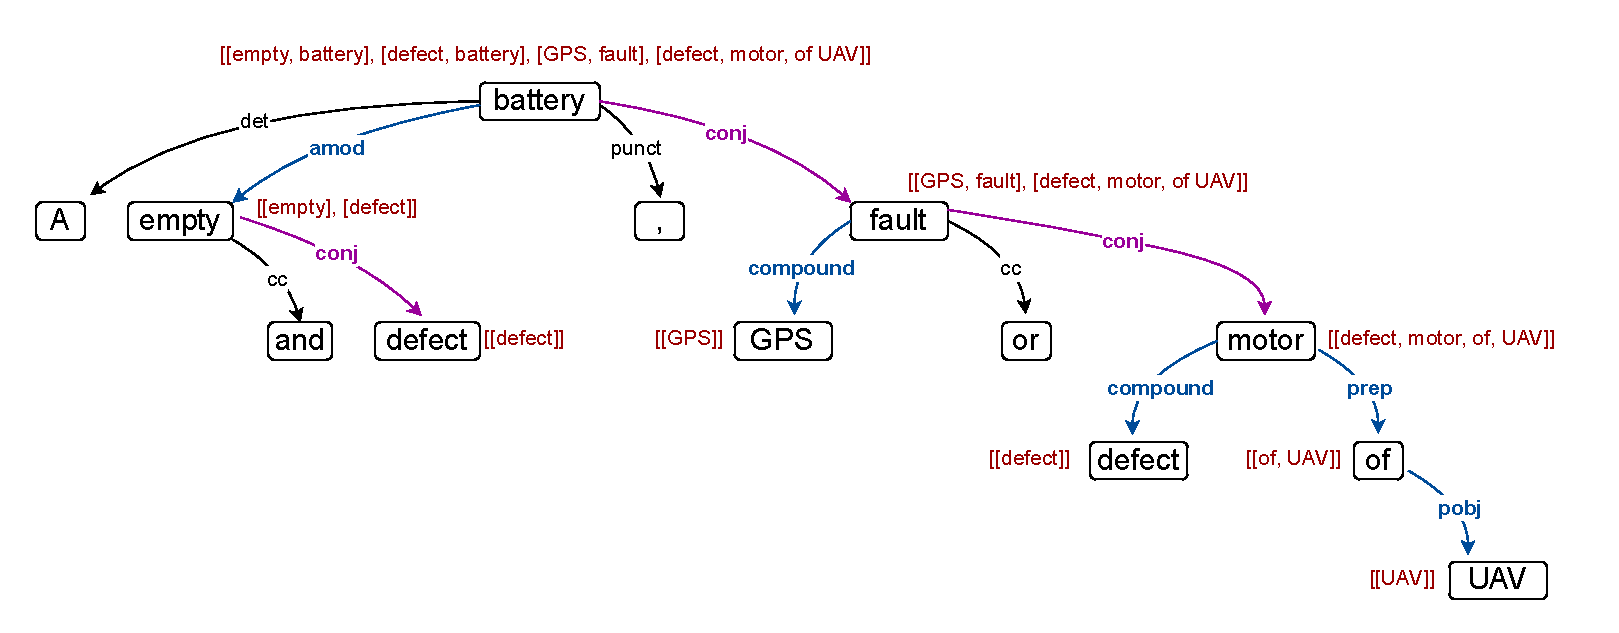
\includegraphics[width=\textwidth]{figures/cause_effect_extraction/phrase_algoirthm_example}
    \caption{Phrase Extraction Algorithm Example}\label{fig:phrase-example}
\end{figure}


In \autoref{alg:phrase-pseudocode} we can see the pseudocode for the phrase extraction algorithm.
The algorithm takes a single token as input and returns multiple phrases.
Thus, it returns a list of lists, where the outer list defines the multiple phrases and the inner lists consist of the tokens in a phrase.
Our recursive algorithm follows the dependency\footnote{Add the dependencies here} links from the input token based on a predefined list of dependencies.
We extend the dependencies from \cite{sharp2016creating} to handle multiple phrases.
In \autoref{fig:phrase-example}, we can see the dependency tree for the sentence \qq{A empty and defect battery, GPS fault or defect motor of UAV causes a crash.}.
This example shows a dependency tree and each interim recursion result at the node level.
The recursion stops at the leaf level of the dependency tree.
We defined the recursion base case by returning a list of a single phrase containing only the leave token (lines 2 to 4).
After defining the base case in the recursion, we need to define how to handle the merge approach.
We have three different cases that we need to handle.
We use the variable phrases (line 5) to store the results from the different cases.
The first case handles all the children linked with a dependency link from the list to the parent node (lines 6 to 15).
We first apply the recursion step to each child token (lines 8 to 11).
We then reduce the different phrases from the tokens into a single list (line 12).
We do so by using the cartesian product between two lists and the results list from the children as input in a higher-order reduce function.
These operations produce multiple phrases that cover all combinations of the phrases from the children.
The last step is to insert the root token into each phrase and sort each phrase based on the occurrence of a token in the sentence (line 13).
We then add the resulting phrases into the phrases variable (line 14).
The second case occurs when the token has no child connected with a dependency from the list line (15 to 17).
We then simply need to add the single token to the phrases list.
An example of why we need this can be seen for the node \qq{empty} in the figure.
Without the previous case, we would not include \qq{empty} in the resulting phrases because there are no children results where we can merge the token into.
The last case (lines 18 to 21) handles the conjunctions dependencies.
Finally, we apply the recursion step for each child that is connected by a conjunction with the token.
With this novel recursive algorithm, we were able to extract four phrases from the example sentence: \qq{empty battery}, \qq{defect battery}, \qq{GPS fault} and \qq{defect motor of UAV}.


\section{Filter Noise Phrases}\label{sec:filter-noise-phrases}
In the previous step, we were able to identify multiple phrases from a single root token.
However, during this expansion, the phrases can contain noise and vague information.
Thus, some phrases need to be filtered or shortened.
We defined that a complete phrase needs to include either a VERB, PROPN, or a NOUN. If a phrase does not contain a token that has such a \ac{POS} tag, we drop the phrase.
We then removed all tokens with the PRON tag such as \qq{I}, \qq{we} or \qq{they}.
Next, we created a list of lemmas e.g., \qq{by}, \qq{any} or \qq{which}, which was manually created by analyzing the extracted phrases.
Finally, we removed the start and end tokens from the phrases based on that list.
Thus, we now have cleaned phrases that can be used to create \ac{CEP}s.


\section{Combine Phrases To Cause-Effect Pairs}\label{sec:combine-the-phrases-to-a-pair}
In \autoref{sec:phrase-extraction} and \autoref{sec:filter-noise-phrases}, we extract and filter phrases based on a single root token.
We use these approaches to find the phrases for the root cause and the root effect in a sentence that we find by applying the patterns from \autoref{sec:dependency-matching}.
The final step is to create \ac{CEP}s from these phrases by combining the phrases with the cartesian product.
In the example sentence from \autoref{sec:phrase-extraction} the root cause was \qq{battery} and the root effect \qq{crash}.
We were able to extract four phrases from \qq{battery} and one phrase from \qq{crash}.
By applying the cartesian product between the phrases we get the \qq{CEP}s: \qq{empty battery} => \qq{crash}, \qq{defect battery} => \qq{crash}, \qq{GPS fault} => \qq{crash} and \qq{defect motor of UAV} => \qq{crash}.

    \chapter{Causal Graph}\label{ch:causal-graph}
In this chapter, we want to provide a methodology to generate a \ac{WDCG} from \ac{CEP}s, as well as for the flight logs dataset.
The nodes in the \ac{WDCG} consist of the phrases, and the edges represent a causal relation between two nodes.
The edges also contain a numerical weight that represents the occurrence of such relationships in the source.
We also provide a tool that visualizes such \ac{WDCG} and allows to interactively examine the graph.


\section{Graph From Cause-Effect Pairs}\label{sec:graph-from-cause-effect-pairs}
\begin{figure}
    \begin{center}
        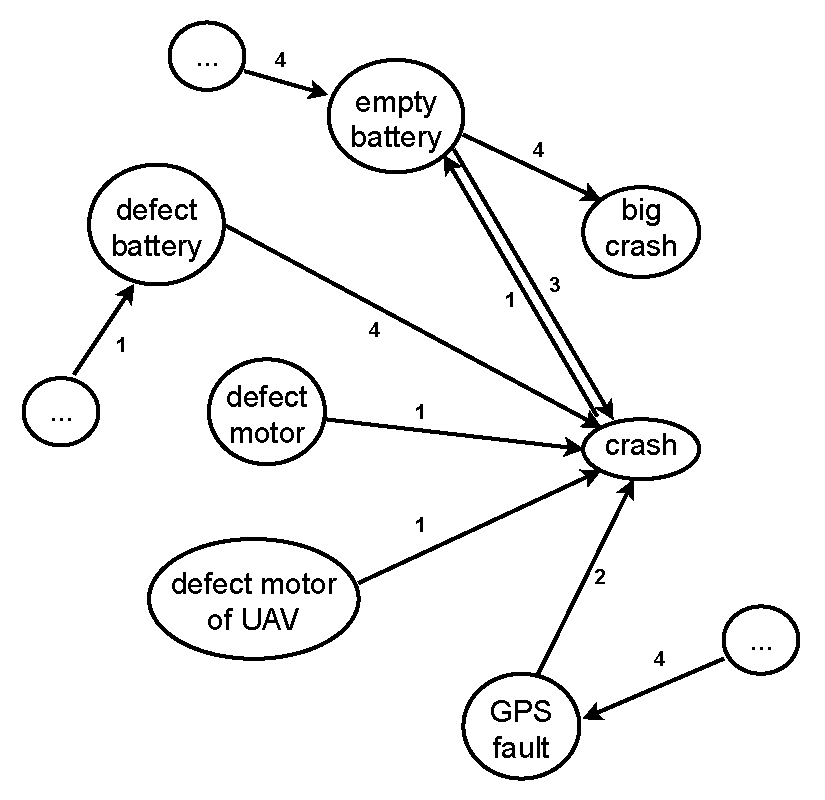
\includegraphics[scale=.6]{figures/causal_graph/causal_graph}
        \caption{Weighted Directed Causal Graph}\label{fig:causal-graph}
    \end{center}
\end{figure}
The previous pipeline step produced multiple \ac{CEP}s.
However, different users may use different words to mean the same thing.
Thus, one user could say \qq{GPS fault causes crash} another would say \qq{GPS error causes crash} so that the cause would be \qq{GPS fault} and \qq{GPS error}.
We used the idea from \cite{Hassanzadeh19} to create a synonym dictionary to replace similar words with a matching synonym in the dictionary
We first created a dictionary that counts all the unique tokens that appear in the \ac{CEP}s, which we sorted in descending order based on the occurrence.
The dictionary indicates the rank of each word in the corpus.
The first element of the dictionary represents the word that the users mostly use.
We then replaced each token of the \ac{CEP}.
To do so, we first used the wordnet corpus to find a list of synonyms for the tokens.
then loop through the sorted dictionaries from high to low occurrence and search for a matching synonym.
Such a hit represents either the same token or a synonym used more frequently by the domain experts.
If we hit such a synonym, we replace the token in the phrase with the synonym.
By following this approach for all phrases in the \ac{CEP}s, we produce a generalized representation of the \ac{CEP}s.
To build the \ac{WDCG} we are merging the same \ac{CEP}s into one \ac{CEP} with a weight attribute that represents the occurrence.
The \ac{CEP} with the weight describes two nodes in the graph, where the cause node has a directed weighted edge to the effect node
We build the \ac{WDCG} by merging the same nodes.
In \autoref{fig:causal-graph} we can see the resulting graph with some additional nodes and edges for the sentence \qq{A empty and defect battery, GPS fault or defect motor of UAV causes a crash}.


\section{Graph From Flight Logs Dataset}\label{sec:graph-from-flight-logs-dataset}
Unfortunately, there is no ground truth graph that we could validate our causal graph.
This section aims to provide the necessary steps to transform the provided flight logs dataset into a \ac{WDCG}.
We will use the resulting graphs in the \autoref{ch:evaluation-methods} module to evaluate the causal graph from the domain-experts with this graph.

\subsection{Flight Logs Dataset}\label{subsec:flight-logs-dataset}
\begin{table}
    \begin{center}
        \label{fig:verb-list}
        \begin{tabular}{||c c||}
            \hline
            ID & DICT \\ [0.5ex]
            \hline\hline
            16 & ekf check        \\
            \hline
            9  & failsafe fence   \\
            \hline
            9  & failsafe fence   \\
            \hline
            9  & failsafe fence   \\
            \hline
            16 & ekf check        \\
            \hline
            17 & failsafe ekfinav \\
            \hline
            16 & ekf check \\ [1ex]
            \hline
        \end{tabular}
    \end{center}
    \caption{\label{tab:flight-log-example-error-table}Flight log example error table}
\end{table}
The flight logs dataset contains thousands of flight logs.
Each flight log contains multiple time series tables, which represent a specific component in the UAV system, which logs the state of the attributes of such component by time.
For example the table \qq{EKF2} represents the \qq{EKF2 Estimation System} with different states such as \qq{attitude},  \qq{velocity'} or  \qq{position} as well as a \qq{timestamp}.
For the scope of the thesis, we will only consider the \qq{EV} and \qq{ERR} tables, which represent the  \qq{Event Subsystem} and the \qq{Error Subsystem}.
In \autoref{tab:flight-log-example-error-table} we can see such a table for the \qq{Error Subsystem}.
The origin table only consists of the ID column.
The DICT column represents the textual representation of the ID. ArduPilot provides a dictionary that maps these IDs into text, which can be found on GitHub \footnote{\url{https://github.com/ArduPilot/ardupilot/blob/master/libraries/AP\_Logger/AP\_Logger.h\#L94}}.
For example, the ID with the value \qq{17} represents \qq{FAILSAFE\_EKFINAV}.
To compare such a label, we decided to split it and used the lowercase representation of the words.
Thus, we would use \qq{failsafe ekfinav} instead of \qq{FAILSAFE\_EKFINAV} as the label.

\subsection{Transforming Into Causal Graph}\label{subsec:transforming-into-causal-graph}
To generate a causal graph from the flight logs data, we applied five steps:
\begin{enumerate}
    \item Create causality chain: We transform the time series tables (\qq{EV} and \qq{ERR}) of the flight logs into a chain of IDs, which is created in the time direction.
    Thus, in our example \autoref{tab:flight-log-example-error-table} we would generate the following chain \qq{16=>9=>9=>. . . =>9=>16=>17=>16}.
    This chain represents the different states of the subsystem in chronological order.
    \item Drop duplicate neighbors: We can see that such chain many of the same links can occur in succession because for these timestamps, the state did not change.
    Thus, we decided to drop such duplicates because they did not add information.
    The chain from the previous step would be processed to the chain \qq{16=>9=>16=>17=>16}.
    \item To structure the chain into a list of \ac{CEP}s, we extracted for each chain item the direct successor.
    Thus, we would extract \qq{16=>9}, \qq{9=>16}, \qq{16=>17}, \qq{17=>16} from the previous chain as \ac{CEP}s.
    This is our assumption, and we are aware that it is not correct in many cases.
    We do this to illustrate how validation could be done if we had ground truth graphs.
    By following steps 1 to 3 for each flight log, we can create a new dataset containing \ac{CEP}s.
    \item Reduce the pairs to a graph: We used the same approach from \autoref{sec:graph-from-cause-effect-pairs} to build a \ac{WDCG} from \ac{CEP}s.
    \item Convert the ids to text: Finally, we translate the numerical ids into textual phrases by using the ArduPilot dictionary.
\end{enumerate}


\section{Data Visualisation}\label{sec:datavisualisation}
To explore the causal graph, we built a visualization tool based on NetworkX\footnote{\url{https://networkx.org/}}, Plotly\footnote{\url{https://plotly.com/}}, and Dash\footnote{\url{https://plotly.com/dash/}}.
NetworkX is a python package for the creation and manipulation, and study of the structure of complex networks, like our causal graph.
We use this package to calculate the position of the nodes of the graph by using a Fruchterman-Reingold force-directed algorithm.
The algorithm holds nodes with treating edges close while treating nodes as repelling objects.
To visualize the graph, we use Plotly, which is an open-source graphing library that allows us to create interactive graphs by using different types of plots.
However, the Plotly library does not natively have an interface to build a directed graph.
To overcome this, we used a scatter plot, where the dots represent the nodes of the graph.
We decided not to draw edges in the default mode because such a graph can potentially have thousands of nodes and edges, which leads to the fact that the edges are not recognizable.
We used color scales to indicate nodes with high connectivity, which is useful to discover the graph.
Fortunate, Plotly allows us to interact with the graph, which is especially useful when dealing with a high amount of nodes.
To get information on the current node, we added a hover functionality that displays the name of the node as well as the name of the predecessors and successors of the node.
To discover the structure in a visual way, we can click a node, which draws all the edges as arrows that are related to the node.
We also added annotations that show the name of these nodes.
We used Dash to create an interactive web application, which runs the Plotly graph in the web browser.

    \chapter{Evaluation Methods}\label{ch:evaluation-methods}
The last step of the pipeline is to evaluate the results in an automatic way.
We first want to provide a methodology to measure the performance of the \ac{CEP} extraction algorithm.
Second, we want to provide methodologies to evaluate the overall quality of the \ac{WDCG} by using different quality scores.


\section{Performance Measurement Of Cause-Effect Pair Extraction}\label{sec:measure-the-performance-of-the-cause-effect}
In this section, we want to provide a methodology to create a dataset consisting of sentences labeled with multiple \ac{CEP}s.
We then use the performance measurement method from \cite{pawar2021knowledge} as a baseline, which can handle a dataset where each sentence can only have one \ac{CEP}.
We first want to improve the definition of their \qq{matching} criteria by computing the \ac{IoU} between a predicted and labeled \ac{CEP} and deciding based on a threshold value if the pair is \qq{matching}.
We second extend the idea to measure the performance of multiple \ac{CEP}s in the same sentence.

\subsection{Datasets}\label{subsec:datasets}
\begin{figure}
    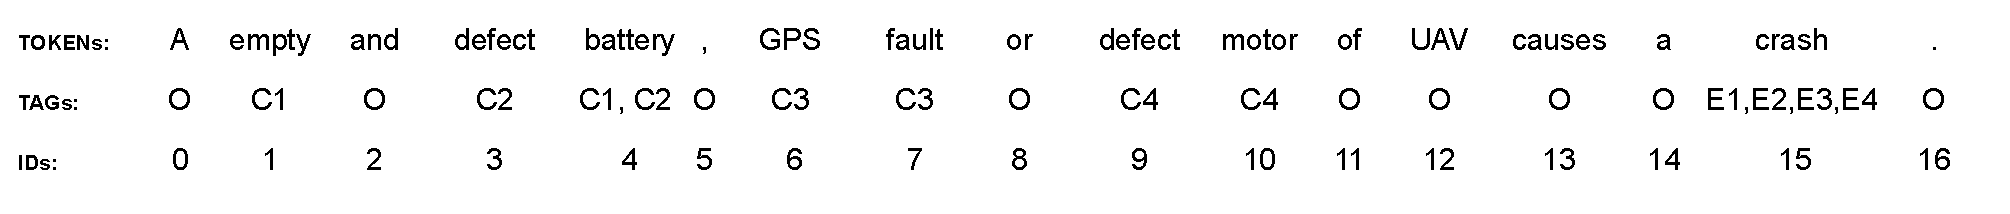
\includegraphics[width=\textwidth]{figures/evaluation_methods/labled_dataset}
    \caption{Labeled Sentence Example}\label{fig:labeled-sentence}
\end{figure}
In this subsection, we want to describe two benchmark datasets that can be used to measure the performance of a \ac{CEP} extracting algorithm.
We followed the \qq{event sequence block label} method from \cite{xu2020review} to create our benchmark datasets.
In \autoref{fig:labeled-sentence} we can see how such labeling look on the sentence \qq{A empty and defect battery, GPS fault or defect motor of UAV causes a crash}.
This labeling technique splits a sentence into tokens and then assign to each token a specific label which can be either \qq{C} cause, \qq{E} effect, or \qq{O} other.
Moreover, to solve the multiple causality problem, we can assign to the \qq{C} and \qq{E} tag an ID such as \qq{C1} or \qq{E1}, to divide different \ac{CEP}s.

\subsubsection{Nato-SFA Dataset}\label{subsubsec:nato-sfa}
In \cite{Hassanzadeh19}, the authors provided the \ac{NATO-SFA} benchmark dataset, which \qq{examines the main trends of global change and the resultant defense and security implications for NATO}\footnote{\url{https://www.act.nato.int/images/stories/media/doclibrary/171004_sfa_2017_report_hr.pdf}}.
Their dataset contains 118 pairs where the first 59 are \ac{CEP} and the other 59 pairs have no causal relations.
Unfortunately, the authors only provided the extracted pairs and the methodology for extracting these pairs.
Thus their dataset does not provide the source sentences of the pairs.
Furthermore, the authors only handle single \ac{CEP}s.
Therefore, we followed their methodology to create a dataset based on their extractions and the report.
We were able to find 100 sentences that are represented in their dataset.
We then used the tokenizer from spaCy to split the sentence into multiple tokens.
Next, we labeled each token manually based on the pairs from the original dataset.
Furthermore, some of the \ac{CEP}s include conjunction, which we manually divided into independent \ac{CEP}s.
We want to use this dataset to compare our results with a dataset from a different domain with high-quality sentences and less noise.

\subsubsection{ArduPilot Dataset}\label{subsubsec:ardupilot}
To measure the performance of the \ac{CEP} extraction, particular for our domain, we created a dataset based on the sentence we gathered during scraping.
This dataset currently contains 69 sentences, where 20 did not include causation, 32 included a single \ac{CEP} and 17 multiple \ac{CEP}s.
Furthermore, we also included some linguistic features in the dataset.
These could potentially be useful if we want to extend the \ac{CEP} algorithm with a machine learning solution, which uses the linguistic tags as features during training.
In the dataset, we have the following columns:
\begin{itemize}
    \item id - integer: This id represents the unique id from the sentence from which we extracted the token.
    \item token - string: Represents the raw text information of the token.
    \item tag - string: This defines the label of the token (see. \autoref{fig:labeled-sentence})
    \item token\_id - integer: The id of the token in the sentence represents the order of the tokens (see \autoref{fig:labeled-sentence}).
    \item lemma  - string: The lemmatized representation of the token.
    \item pos  - string: The \ac{POS} tag for the token.
    \item dep  - string: The \ac{DEP} tag for the token.
\end{itemize}

\subsection{Performance Measurement}\label{subsec:performance-measurement}
\begin{figure}
    \begin{center}
        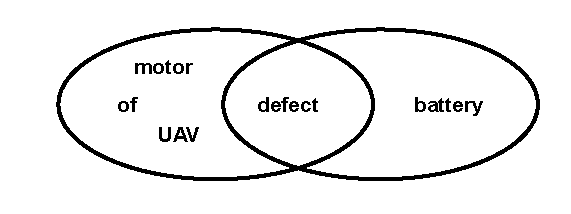
\includegraphics[scale=.85]{figures/evaluation_methods/jaccard_similarity}
        \caption{Jaccard Similarity}\label{fig:jaccard-similarity}
    \end{center}
\end{figure}
In \cite{pawar2021knowledge} the authors defined a match between two \ac{CEP}s when at least one word between the cause phrases is matching as well as between the effect phrases.
Thus, \qq{defect motor of UAV} => \qq{crash} and \qq{defect battery} => \qq{crash} would be matching because \qq{defect} and \qq{crash} are in both phrases.
Instead of using a fixed rule, we want to calculate the \ac{IoU} between two \ac{CEP}s and compare the \ac{IoU} with a threshold value to decide if the \ac{CEP}s are \qq{matching}.
To calculate the \ac{IoU}  between two \ac{CEP}s, we first calculate the \ac{IoU}  between the cause phrases and, accordingly, the effect phrases.
Fortunate, the Jaccard similarity defines the \ac{IoU} between two phrases:
\begin{equation}
    \label{eq:jaccard-similarity}
    J(P1, P2) = \frac{\left| P1 \cap P2 \right|}{\left| P1 \cup P2 \right|}
\end{equation}
In \autoref{fig:jaccard-similarity} we see a graphical representation of the Jaccard similarity between the two phrases \qq{defect motor of UAV} and \qq{defect battery}.
In this example, the Jaccard similarity is $1/5$, thus 0.2. However, the Jaccard similarity between the textual representations of phrases could lead to unintentional errors because we cannot differentiate between textual tokens.
Thus, in our previous example, the \ac{IoU} should be 0 because the \qq{defect} of both phrases represents a different token in the sentence (see \autoref{fig:labeled-sentence}).
To have distinct representations of the tokens, we use the \qq{token\_id} of the labeled dataset and the predictions.
We defined the \ac{IoU} between two \ac{CEP}s by calculating the harmonic mean between the \ac{IoU}  of the cause phrases and the \ac{IoU} of the effect phrases with:
\begin{equation}
    \label{eq:iuo-cause-effect-pair}
    IoU\_CEP(cause\_IoU, effect\_IoU) = 2*\frac{cause\_IoU*effect\_IoU}{cause\_IoU+effect\_IoU}
\end{equation}
After calculating \ac{IoU} between two pairs, we can define the \qq{matching} term by comparing the \ac{IoU}  with a threshold:
\begin{equation}
    \label{eq:matching}
    Matching(IoU, threshold) = \left\{
    \begin{array}{ll}
        True  & IoU > threshold  \\
        False & IoU <= threshold \\
    \end{array}
    \right.
\end{equation}
A \ac{TP} is counted for each labeled pair in the dataset if there is a \qq{matching} predicted pair and a \ac{FN} otherwise.
Also, a \ac{FP} is counted for each predicted pair if there is no \qq{matching} labeled pair in the dataset.
Precision, Recall, and F1-score are computed as follows:
\begin{equation}
    \label{eq:measurement-scores}
    Precision = \frac{TP}{TP+FP}
    \quad\mathrm{,}\quad
    Recall = \frac{TP}{TP+FN}
    \quad\mathrm{,}\quad
    F1 = 2*\frac{Precision*Recall}{Precision+Recall}
\end{equation}
We can now calculate the performance measurement scores on different threshold values, which allows us to create a 2d-plot with threshold values ranging from 0 to 1 on the x-axis and performance scores on the y-axis (see \autoref{ch:results}).


\section{Find Cause-Effect Pairs In The Flight Logs}\label{sec:find-cause-effect-pairs-in-the-uav-logs}
This section provides different quality scores to evaluate the \ac{WDCG}.

\subsection{Graph Matching}\label{subsec:graph-matching}
We want to lay the foundation of the following quality scores in this subsection.
We can perform two types of queries on a \ac{WDCG}.
The first query takes a node as input and responds with the amount of \qq{matching} nodes in the graph.
We can calculate the amount by summing all weights from the edges connected with the search node.
Thus, if we have as input \qq{empty battery}, we would get a total of 12 mentions (see \autoref{fig:causal-graph}).
The second query represents an edge consisting of two nodes, where the response is the weight of all \qq{matching} edges in the graph.
Thus, if we have as input \qq{empty battery} =>\qq{crash} we get a total of 3 mentions returned.
The previous examples represent exact matching between the nodes or edges.
However, if we have an input like \qq{battery} => \qq{crash} the graph did not have the exact representation of the pair.
We want to use the same idea from the previous section to use \ac{IoU} with a threshold value to decide if such a query is \qq{matching}.

\subsection{Diversity Of A Graph}\label{subsec:diversity-of-graph}
We define the diversity of a node by the fraction between the number of explicit mentions and the number of mentions when making a query based on a threshold value.
For example, the node \qq{empty battery} would lead to 12 explicit mentions and 17 mentions with a threshold value of 0.6 because we also count the mentions for \qq{defect battery}.
The diversity can be defined as follows:
\begin{equation}
    \label{eq:node-diversity}
    node\_diversity(thresh) = \frac{exact\_node\_mentions}{node\_mentions(thresh)}
\end{equation}
\begin{equation}
    \label{eq:edge-diversity}
    edge\_diversity(thresh) = \frac{exact\_edge\_mentions}{edge\_mentions(thresh)}
\end{equation}
Thus for the node \qq{empty battery} we would have a diversity of $12/17=0.706$ at threshold 0.6.
The diversity ranges from 0.0 to 1.0, where 1.0 indicates that no other representation for this information is in the \ac{WDCG}.
A low diversity score indicates multiple nodes with similar meanings.
Thus, the same information in the graph is spread to different nodes.
To calculate the diversity for the whole graph, we calculate the diversity for each node and take its mean.
We can calculate the diversity for different threshold values in a similar to \autoref{subsec:performance-measurement}.
We calculate the diversity for a node and an edge similarly.

\subsection{Consistency Of The Edges}\label{subsec:consistency-of-the-edges}
The consistency score defines the quality of an edge by comparing it with the direct contradiction.
In general if there is a causality like \qq{empty battery} => \qq{crash"} \qq{crash} => \qq{emtpy battery} would be the direct contradiction.
We calculate consistency by first calculating the number of mentions of the edges ($edge\_mentions$)and the number of mentions where we swap the direction of the relation of the edge ($reversed\_edge\_mentions$):
\begin{equation}
    \label{eq:consistency-score}
    consistency(thresh) = \frac{edge\_mentions(thresh)}{edge\_mentions(thresh) + reversed\_edge\_mentions(thresh)}
\end{equation}
Thus if 10 users would say \qq{empty battery} => \qq{crash} and only one user \qq{crash} => \qq{emtpy battery} we would have a consistency score for the first edge of ~''0.91'', whereas for the second edge ~''0.09''.
The consistency score ranges between 0.0 and 1.0, where 1.0 means no contradictions.
A consistency score of 0.5 can be interpreted that the users are not sure about the relation of the nodes.
On the other hand, a score near 0.0 indicates that the majority disagree with this edge.


\subsection{Information Score}\label{subsec:information-score}
We want to provide a measure representing the information value of an edge.
Therefore, we define the information of an edge with:
\begin{equation}
    \label{eq:information-score}
    information(thresh) = consistency(thresh) * edge\_mentions(thresh)
\end{equation}
For example the edge \qq{empty battery} => \qq{crash} would have a information score of $0.91 * 10=9.1$.
This score reflects how often an edge is mentioned and penalties edges that have contradictions.
Based on the information score, we define an edge as valuable with:
\begin{equation}
    \label{eq:value_edge}
    valuable(information) = \left\{
    \begin{array}{ll}
        True  & information > 1  \\
        False & information <= 1 \\
    \end{array}
    \right.
\end{equation}
Thus, an edge can only be valuable when mentioned at least two times.
Furthermore, an edge cannot be valuable when the edge has too many contradictions.

\subsection{Coverage Between Two Graphs}\label{subsec:coverage-between-two-graphs}
The coverage score represents how many nodes/edges are reflected in a target graph.
To calculate the score, we assign a boolean label to each node/edge in the source graph that indicates if the node/edge is reflected in the target graph.
The coverage score for the graph is the fraction between the number of true labels and the number of the total nodes/edges.
Thus, if we have a source graph of 1000 nodes and a target graph of 50 nodes where 25 nodes match both, we would have coverage of \qq{2,5\%} for the source graph and \qq{50\%} for the target graph.

\subsection{Correctness Of Graph}\label{subsec:correctness-of-graph}
The correctness of the causal graph can be measured by considering the flight log graph as the ground truth.
We assign a correct label to each edge, which can be \qq{correct}, \qq{incorrect}, or \qq{unknown} based on the valuable label.
We use the edge from the source graph as the input for the matching query on the target graph to find if the edge is also detected as valuable in the target graph.
We define the edge as \qq{unknown} if the \qq{information} of the target graph is 0 because there is no evidence in the target graph, which means that we cannot deduct the correctness of the edge.
However, if there is evidence in the target graph, we define the edge as correct if the edge is valuable in the source graph and the target graph; otherwise, we define it \qq{incorrect}.
To calculate the correctness of the whole causal graph, we use:
\begin{equation}
    \label{eq:correctness}
    correctness(thresh) = \frac{correct\_edges(thresh)}{correct\_edges(thresh) + incorrect\_edges(thresh)}
\end{equation}

    \chapter{Results}\label{ch:results}
In this section, we want to evaluate our results for the \ac{CEP} extraction algorithm, \ac{WDCG} and the overall performance of the End-to-End pipeline.


\section{Performance Of The Cause-Effect Pairs Extraction}\label{sec:performance-measure}
\begin{figure}
    \begin{center}
        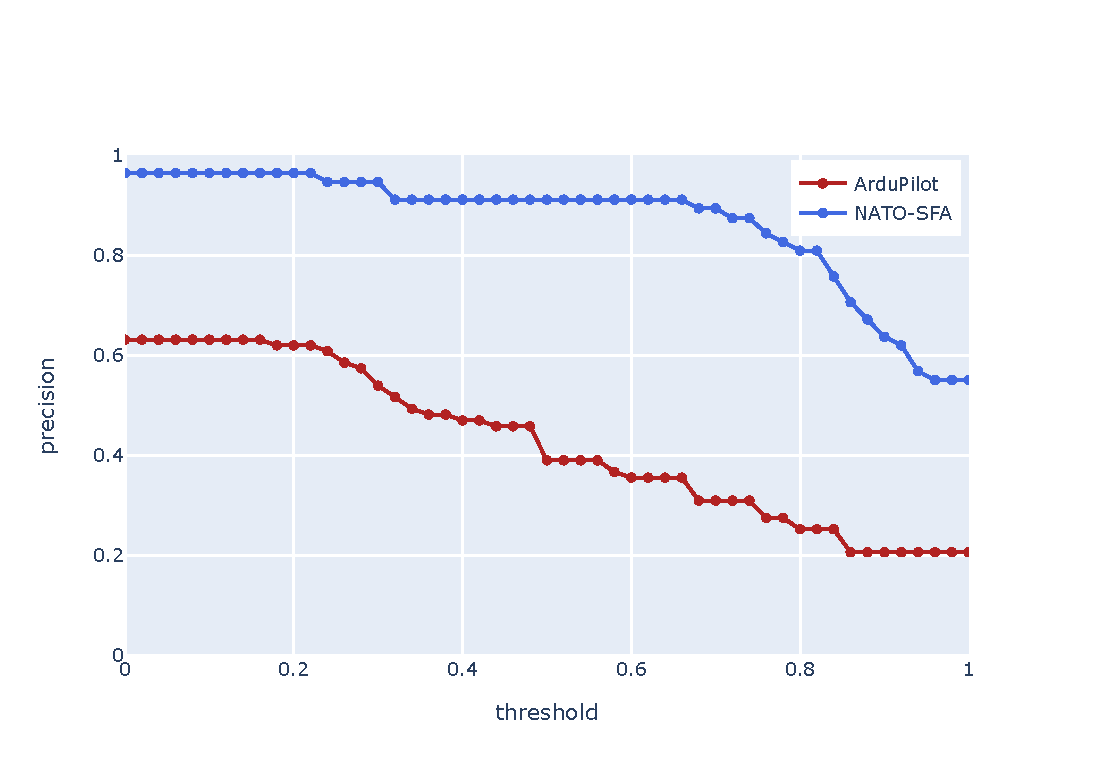
\includegraphics[scale=.65]{figures/results/precision}
        \caption{Precision comparison between ArduPilot and NATO-SFA dataset}\label{fig:precision}
        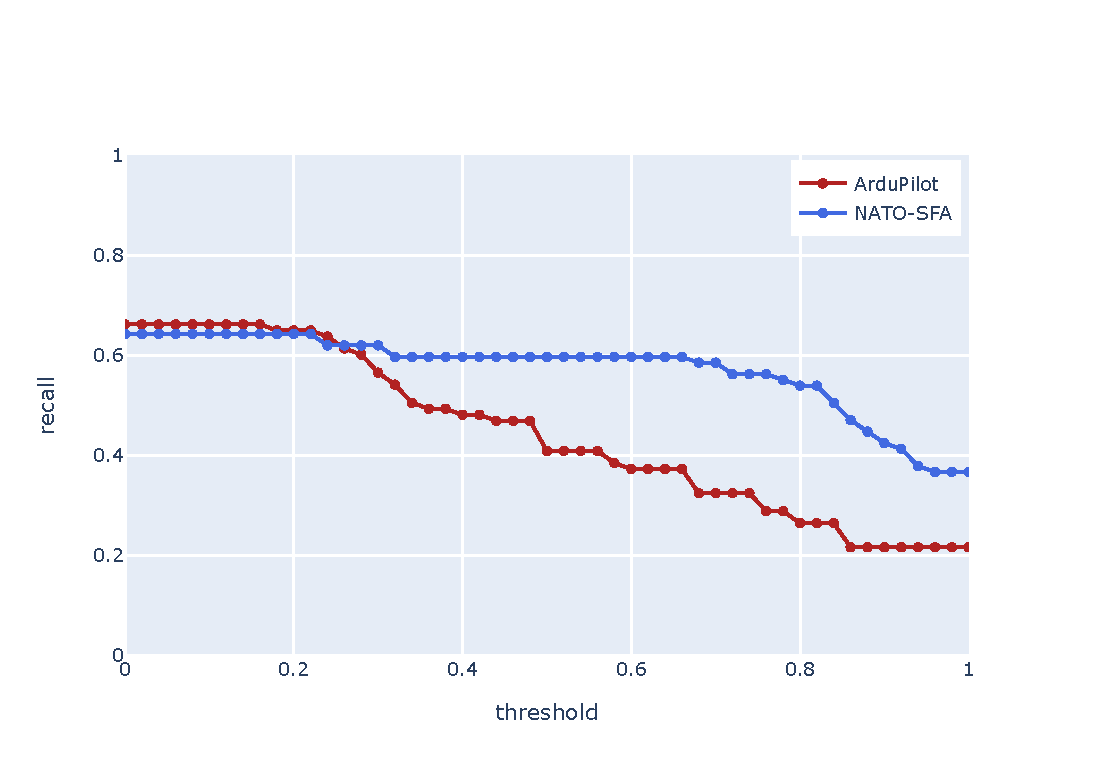
\includegraphics[scale=.65]{figures/results/recall}
        \caption{Recall comparison between ArduPilot and NATO-SFA dataset}\label{fig:recall}
    \end{center}
\end{figure}
In \autoref{fig:precision} and \autoref{fig:recall} we can see the precision and recall of the \ac{CEP} extraction algorithm for the Ardupilot dataset in comparison to the NATO-SFA benchmark dataset.
In addition, the graphs plot the performance scores based on different threshold values (see. \autoref{subsec:performance-measurement}).
We can first notice that the curves are continuously decreasing, that is because, for a higher threshold value, more \ac{CEP}s are not matching.
Thus, the \ac{FP} and \ac{FN} are increasing, which leads to this behavior.
Second, the precision score of the \ac{NATO-SFA} dataset is for each threshold value higher than the precision score of the ArduPilot dataset.
The reason for that is that the \ac{NATO-SFA} dataset consists of shorter sentences with longer phrases, which makes it more likely to hit such a phrase which leads to a \ac{TP}.
In contrast, the recall scores between the datasets are more similar, and only at a threshold value > 0.3 the \ac{NATO-SFA} dataset has a higher recall.
Recall defines how many labeled \ac{CEP}s we are hitting.
Thus, we can say that the algorithm we provide is general in detecting \ac{CEP}s.
In \autoref{fig:recall} the authors achieved with comparable dependency patterns, but without handling multiple \ac{CEP}s and conjunctions a precision of \qq{0.5083},  recall \qq{0.3566} and f1-score of \qq{0.4191}.
Furthermore, they measured these scores with strict rules for the \qq{matching} term (see \autoref{sec:measure-the-performance-of-the-cause-effect}).
This would be similar for any threshold value greater than zero with our approach.
To compare their results with ours, we use the threshold value of 0.01.
We achieved a precision \qq{0.6322}, recall \qq{0.6626} and f1 \qq{0.6471} at the ArduPilot dataset.
Thus we were able to improve the performance measurements with our approach.
Furthermore, we were able to have even a better precision for threshold vales < 0.32 and a better recall for threshold values < 0.66.
Additionally we achieved a precision \qq{0.9655}, recall \qq{0.6437} and f1 \qq{0.7724} score on the \ac{NATO-SFA} dataset.
Thus our method of extracting multiple \ac{CEP}s is well-performing.


\section{Causal Graph Evaluation}\label{sec:causal-graph-evaluation}
\begin{table}
    \begin{center}
        \begin{tabular}[t]{||c c c||}
            \hline
            cause                & effect                        & weight \\ [0.5ex]
            \hline\hline
            problem              & crash                         & 8      \\ \hline
            wing                 & lift                          & 6      \\ \hline
            ap                   & camara                        & 5      \\ \hline
            auto mode            & kickstart acceleration        & 4      \\ \hline
            parameter            & problem                       & 4      \\ \hline
            motor                & thrust                        & 4      \\ \hline
            vibration            & problem                       & 4      \\ \hline
            right step regulator & fix output from input voltage & 4      \\ \hline
            transmitter          & follow control change         & 3      \\ \hline
        \end{tabular}
        \caption{Mostly mentioned edges from the ArduPilot graph}\label{tab:table-base-on-weight}
    \end{center}
\end{table}
In this section, we want to show the results for the ArduPilot graph and then evaluate them in comparison to the generated flight logs graph.
The ArduPilot graph consists of 3941 unique nodes with 3301 edges, where 3180 of the edges have a weight of 1, which means that only one user mentioned exactly such an edge.
The other 121 edges are mentioned multiple times by different users and have a total weight of 280.
In \autoref{tab:table-base-on-weight} we can see the edges listed in descending order based on their weight.
For example, the highest weight of 8 has the \ac{CEP} \qq{problem}=>\qq{crash}.
We can see that the pairs mentioned multiple times are generic phrases without much additional information and often contain only one word.
However, the mean of the word count in a node is \qq{2.763} words per node because edges with lower weight tend to include more information and are more specific.
On the other hand, the flight logs graph contains 26 nodes, 220 edges, and a total of 9904 weight, which represents a more dense graph.
This graph contains a small number of nodes due to the limitations of the dataset.

\subsection{Diversity In The Online Resources}\label{subsec:how-diverse-are-the-mentioned-cause-and-effect-events-in-the-online-resources?}
\begin{figure}
    \begin{center}
        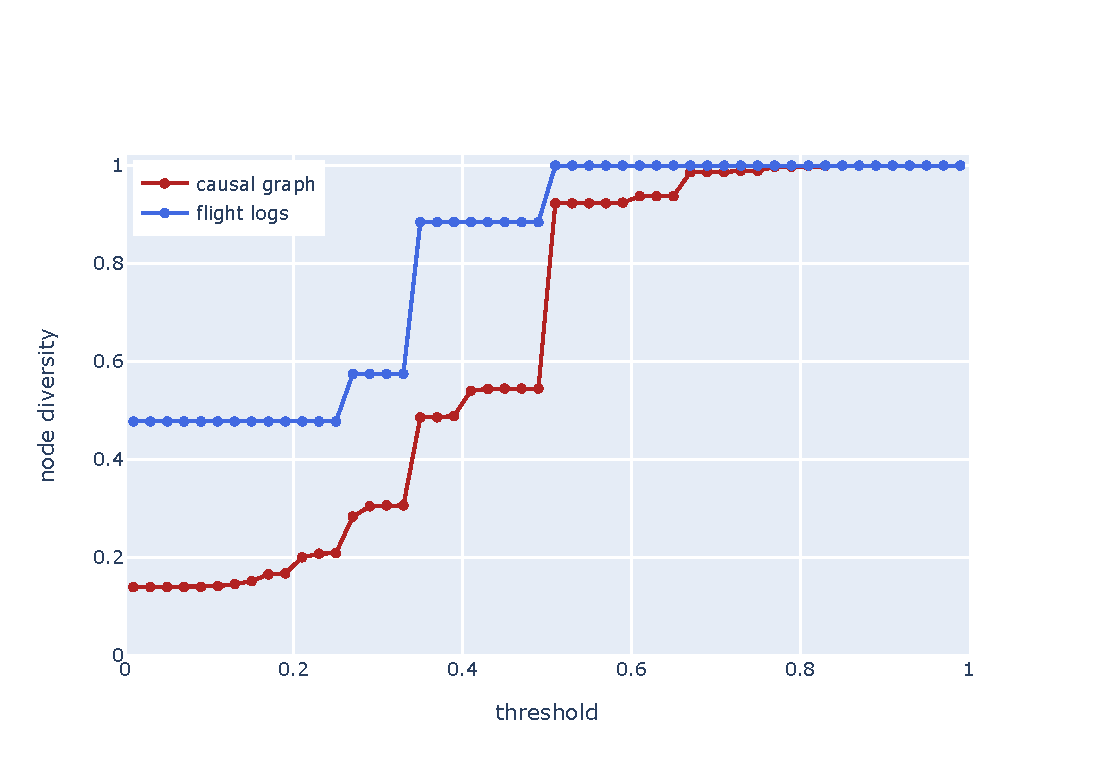
\includegraphics[scale=.65]{figures/results/node_diversity}
        \caption{Node diversity}\label{fig:node-diversity}
        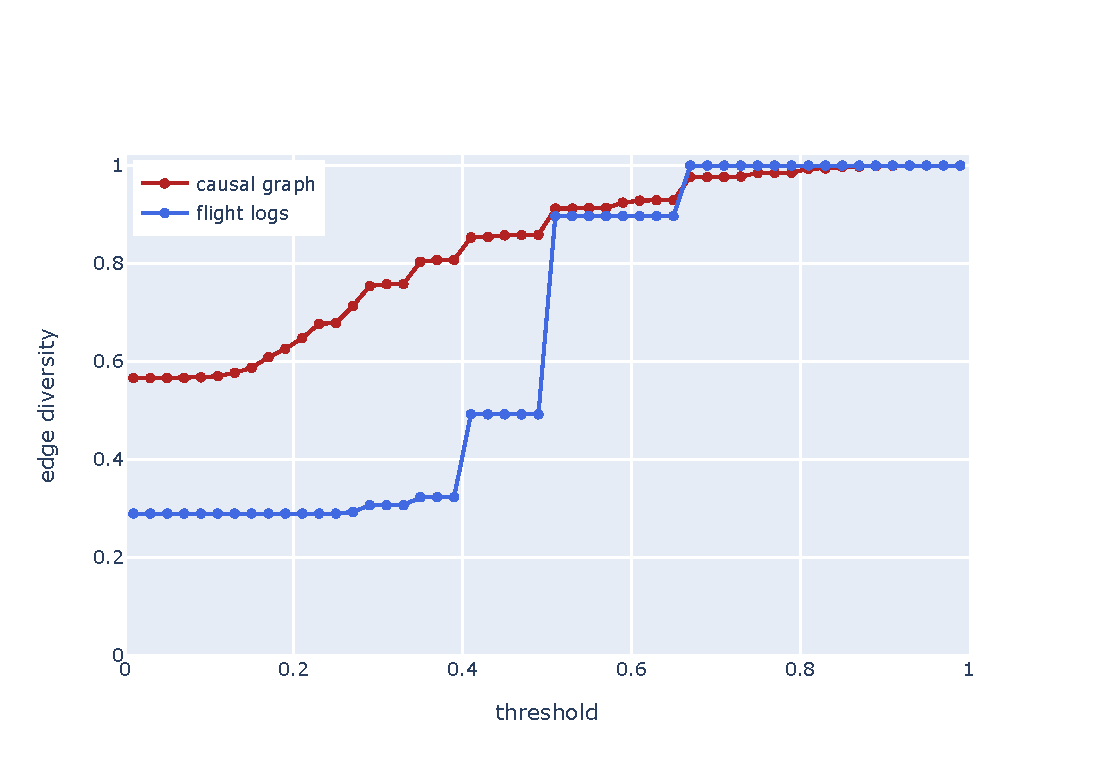
\includegraphics[scale=.65]{figures/results/edge_diversity}
        \caption{Edge Diversity}\label{fig:edge-diversity}
    \end{center}
\end{figure}
In \autoref{fig:node-diversity} we can see the diversity of the nodes from the causal graph and the flight logs.
Moreover, the diversity plot has the characteristic that it increases and converges to 1.0 (see. \autoref{subsec:diversity-of-graph}).
Furthermore, we can see that the diversity makes a vast jump around the 0.5 threshold value.
The reason for that is our similarity score (see. \autoref{eq:jaccard-similarity}).
The node similarity for the causal graph is low, which means that many nodes contain similar information.
For example, we were not able to merge the node \qq{crash}, \qq{big crash} or \qq{crash of UAV} into one node.
The flight logs have a higher diversity in comparison to the causal graph.
The diversity of nodes represents the language in the graph and describes how often the users use a similar term or phrase to describe a problem without the context of the relations.
The node diversity of the online resource is comparatively low, meaning that users use the same language or information to explain the problems.
In \autoref{fig:edge-diversity} we can see the diversity for the edges from the causal graph and the flight logs.
We can see that the edge diversity for the causal graph is higher than the node diversity because the users are more likely to express the same \ac{CEP} with different information.

\subsection{Consistency In The Online Resource}\label{subsec:consistency-question}
\begin{figure}
    \begin{center}
        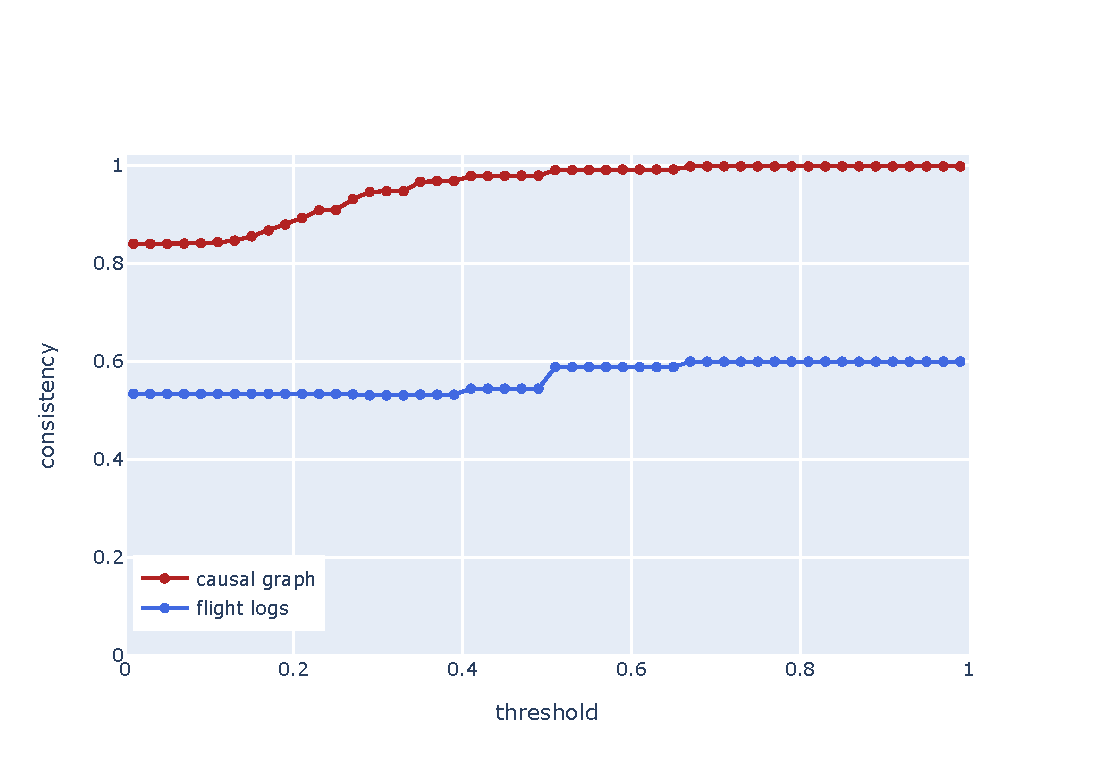
\includegraphics[scale=.65]{figures/results/consistency}
        \caption{Consistency}\label{fig:consistency}
    \end{center}
\end{figure}
In \autoref{fig:consistency} we can see the consistency plot of the causal graph and the flight logs graph.
The consistency of the causal graph is pretty high, even on a low threshold value.
Thus, we can say that the Ardupilot community is consistent in its knowledge, and the edges in the graph do not contain many contradictions.
The flight logs have a consistency score near 0.5 which means that there are a lot of \qq{ekf check} => \qq{failsafe fence} and \qq{failsafe fence} => \qq{ekf check} contradictions.
The reason for that is the way we generate the graph.
We modeled the time series data in a repeating events or errors chain.
However, building it that way was the only possible method to build a comparable graph from another resource.

\subsection{Detectability Between The Graphs}\label{subsec:coverage-question}
\begin{figure}
    \begin{center}
        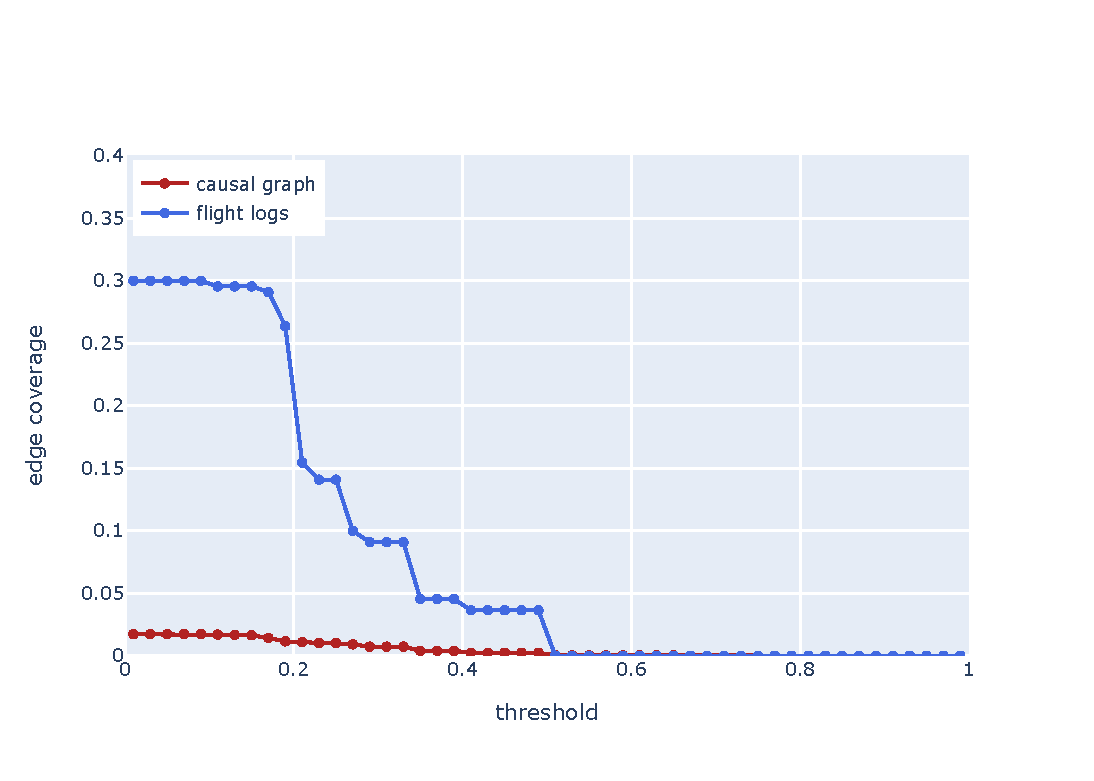
\includegraphics[scale=.65]{figures/results/edge_coverage}
        \caption{Coverage Edges}\label{fig:coverage_edge}
        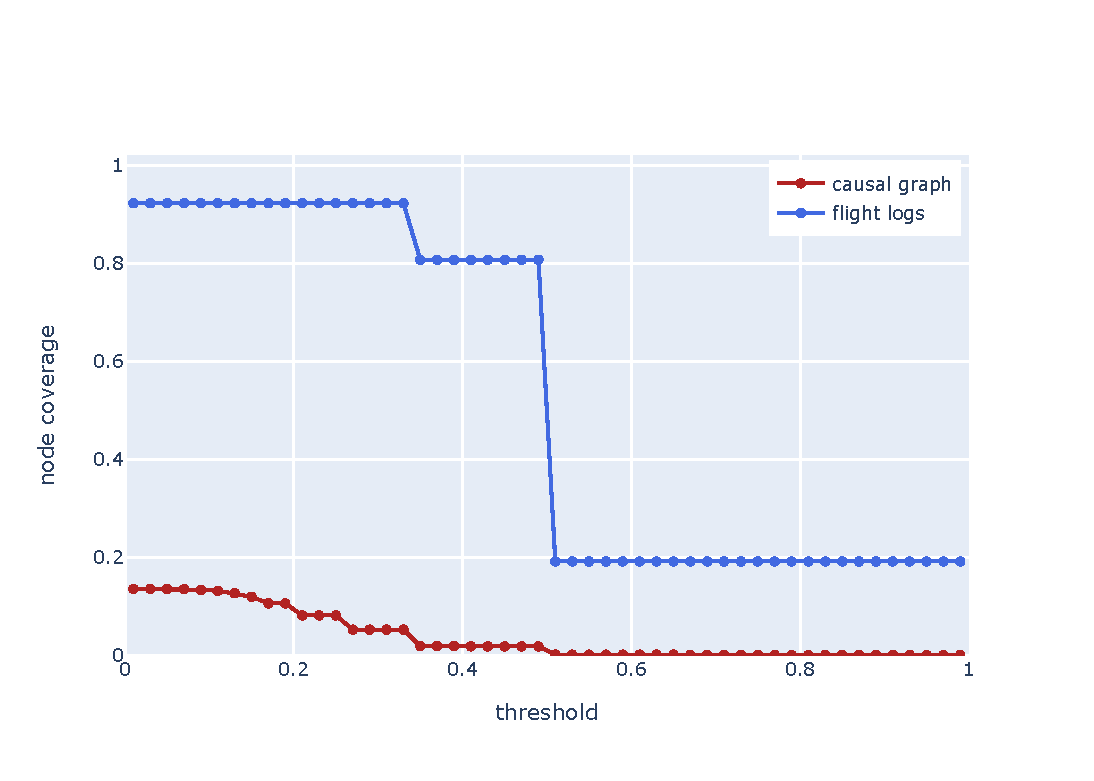
\includegraphics[scale=.65]{figures/results/node_coverage}
        \caption{Coverage Nodes}\label{fig:coverage_node}
    \end{center}
\end{figure}
In \autoref{fig:coverage_edge} and \autoref{fig:coverage_node} we can see the graph for the coverage of the nodes and edges of the causal graph and the flight logs.
The coverage for the edges of the causal graph is pretty low and only detectable on a threshold < 0.67.
The highest coverage is at the lowest threshold value, with \qq{1,73}\%.
We can first deduce that there are no exact representations of the \ac{CEP}s from the ArduPilot community and the flight logs.
Second, there are many \ac{CEP}s that the users mentioned and are not reflected in the flight logs.
This is not surprising because the flight log dataset is limited.
We can also see in the \autoref{fig:coverage_edge} figure that the coverage of the edges for the flight logs dataset is on the lowest threshold value \qq{29,6}\%.
Furthermore, we can see that the coverage score for the nodes is higher than the coverage score for the edges.
The node coverage score for the flight logs is pretty high, which means that the users mention much information that can be found in our data.

\subsection{Accuracy Of The Causal Graph}\label{subsec:accurate-question}
\begin{figure}
    \begin{center}
        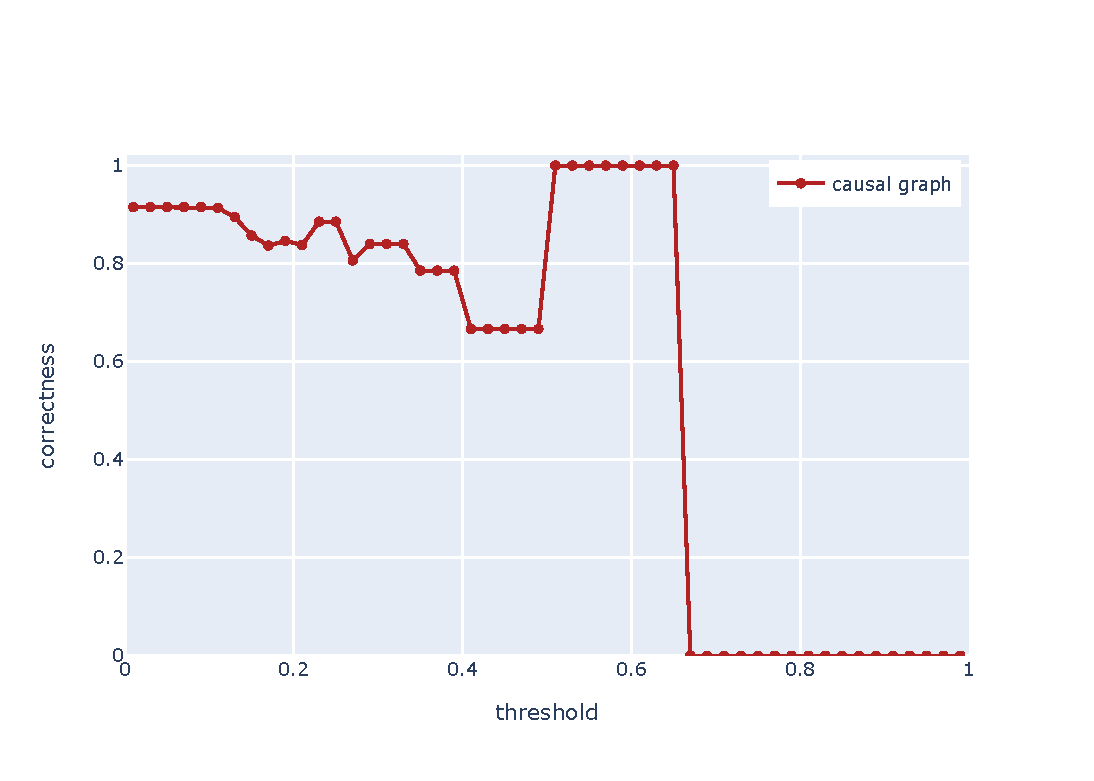
\includegraphics[scale=.65]{figures/results/correctness}
        \caption{Correctness}\label{fig:correctness}
    \end{center}
\end{figure}
The last question we want to answer is the accuracy based on the historical data.
We want to know if the graph represents correct knowledge.
Thus we need a ground truth graph to compare, like the flight logs graph.
In \autoref{subsec:coverage-question} we saw that there are few intersections between the causal graph and the flight logs.
There could be two possible reasons for that.
The first is that the knowledge of the ArduPilot community is incorrect.
The second reason could be that the ArduPilot community provides correct knowledge that is not reflected in the dataset.
We want to use the correctness score from \autoref{eq:correctness} to calculate the correctness of the domain expert knowledge graph.
Remember, the score near one indicates that a \ac{CEP} that a user mentioned is backed with the ground truth data.
In \autoref{fig:correctness} we can see the plot of the score.
The spice in the graph is correlated to the Jaccard similarity we used.
We can only calculate the correctness if there are intersections between the graphs.
Thus we do have correctness of 0 for a threshold >= 0.67 (see subsec:coverage-question).
However, the average correctness score for a threshold < 0.67 is \qq{86.51}\%.
Therefore, we can say that for the \ac{CEP}s that are reflected in the flight logs, we know that they are mostly correct.

\subsection{Mentionable Edges In The Causal Graph}\label{subsec:information-question}
\begin{table}
    \begin{center}
        \begin{tabular}[t]{||c c c c||}
            \hline
            thresh & cause                        & effect                       & info \\ [0.5ex]
            \hline\hline
            0.25   & prop motor                   & pound of thrust              & 35.027 \\ \hline
            0.25   & high vibration               & flight problem               & 32.111 \\ \hline
            0.25   & position of camara           & problem                      & 29.25  \\ \hline
            0.25   & high value                   & crosstrack problem vibration & 29.032 \\ \hline
            0.25   & combination of high altitude & problem                      & 28.488 \\ \hline
            0.25   & quad motor                   & more thrust                  & 27.000 \\ \hline
            0.25   & vibration                    & problem in gqs mode          & 26.281 \\ \hline
        \end{tabular}
        \caption{Mentionable Edges with threshold of 0.25}\label{tab:information-score-25}
        \begin{tabular}[t]{||c c c c||}
            \hline
            thresh & cause          & effect  & info \\ [0.5ex]
            \hline\hline
            0.50   & vibration      & problem & 19.000             \\ \hline
            0.50   & motor          & thrust  & 17.000             \\ \hline
            0.50   & failsafe       & rtl     & 13.000             \\ \hline
            0.50   & problem        & crash   & 11.267             \\ \hline
            0.50   & radio failsafe & rtl     & 10.000             \\ \hline
        \end{tabular}
        \caption{Mentionable Edges with threshold of 0.50}\label{tab:information-score-50}
        \begin{tabular}[t]{||c c c c||}
            \hline
            thresh & cause                            & effect                        & info \\ [0.5ex]
            \hline\hline
            0.75   & problem                          & crash                         & 7.111 \\ \hline
            0.75   & wing                             & lift                          & 6.000 \\ \hline
            0.75   & ap                               & camara                        & 5.000 \\ \hline
            0.75   & auto mode                        & kickstart acceleration        & 4.000 \\ \hline
            0.75   & certain combination of telem1 rx & boot                          & 4.000 \\ \hline
            0.75   & right step regulator             & fix output from input voltage & 4.000 \\ \hline
        \end{tabular}
        \caption{Mentionable Edges with threshold of 0.75}\label{tab:information-score-75}
    \end{center}
\end{table}

\begin{table}
    \begin{center}
        \begin{tabular}[t]{||c c c c||}
            \hline
            thresh & cause                  & effect              & info \\ [0.5ex]
            \hline\hline
            0.25   & compass problem        & crash               & 15.429 \\ \hline
            0.25   & failure of gps compass & crash               & 13.136 \\ \hline
            0.25   & short failsafe issue   & other mode          & 13.000 \\ \hline
            0.25   & gps problem            & land mode problem   & 12.000 \\ \hline
            0.25   & short failsafe issue   & mode change         & 11.077 \\ \hline
            0.25   & ekf failsafe           & change to land mode & 11.000 \\ \hline
            0.25   & gps problem            & flight problem      & 10.083 \\ \hline
        \end{tabular}
        \caption{Mentionable Edges with threshold of 0.25 and the correct label}\label{tab:information-score-25-correct}
        \begin{tabular}[t]{||c c c c||}
            \hline
            thresh & cause           & effect & info \\ [0.5ex]
            \hline\hline
            0.50   & compass problem & crash  & 10.563 \\ \hline
            0.50   & flight          & crash  & 6.000  \\ \hline
            0.50   & failsafe        & mode   & 4.000  \\ \hline
            0.50   & compass         & crash  & 3.200  \\ \hline
            0.50   & gps glitch      & ekf    & 2.000  \\ \hline
        \end{tabular}
        \caption{Mentionable Edges with threshold of 0.50 and the correct label}\label{tab:information-score-50-correct}
        \begin{tabular}[t]{||c c c c||}
            \hline
            thresh & cause & effect & info \\ [0.5ex]
            \hline\hline
            0.75   & -     & -      & -    \\ \hline
        \end{tabular}
        \caption{Mentionable Edges with threshold of 0.75 and the correct label}\label{tab:information-score-75-correct}
    \end{center}
\end{table}

We used the information score to sort all edges in descending order to find the most valuable edges in the causal graph.
In \autoref{tab:information-score-25}, \autoref{tab:information-score-50} and \autoref{tab:information-score-75} we can see such edges ranked on three different threshold values.
As we mentioned earlier, a lower threshold value allows edges that contain more information than a generic word to have a higher score which can be seen in \autoref{tab:information-score-25}.
In \autoref{tab:information-score-25-correct}, \autoref{tab:information-score-50-correct} and \autoref{tab:information-score-75-correct} we see the edges ranked by the information score.
However, we only contain edges labeled as correct regarding the flight logs dataset.


\section{Running Time Analysis}\label{sec:end-to-end-performance}
In this section, we want to analyze the overall performance of the End-o-End tool.
For computation, we used a cloud machine with 16GB RAM.
We scraped three different sources of the ArduPilot community.
We scraped 90 MB of raw textual data from the discussion forum, which took about ~17h 32min.
We scraped 9,23 MB from the discord chat in ~23 min and 11,28 MB from the documentation in ~27 min.
The scraping of the forum took that long because we needed to communicate with a web driver and wait on different actions when executing javascript.
After extracting the sentence and combining everything into one source, we found 724.922 sentences where 610.640 were from the forum, 83.577 from the discord chat, and 30.705 sentences from the documentation.
The combination and extraction of the sentences from the different sources took ~4h 12min.
We found 2758 sentences containing causation that the users explicitly mention, where 2322 of them were from the form, 200 from the documentation, and 236 from the discord chat.
We extracted the sentences in ~47min and needed ~22sec to generate the causal graph from the extractions.
It took ~3h 44min to evaluate the system for 50 different threshold values.

    \chapter{Conclusions}\label{ch:conclusions}
In this thesis, we extracted the vast wealth of knowledge online and made it accessible through a causal graph.
We built a system that scrapes the web from several resources, formalizes the knowledge with \ac{NLP}, extracts \ac{CEP}, and constructs an extensive causal graph for the \ac{UAV} domain.
The methods and technologies we used for \ac{CEP} extraction are extendable, allowing others to contribute to the project efficiently and adaptable, allowing us to apply the procedure for other domains.
Many relations in our graph consist of problems and crashes of a \ac{UAV} helping to find root causes of these failures more efficiently.
In addition, with the significant consistency in our results, we built a causal graph that helps to resolve and backtrack an innumerable number of problems regarding \ac{UAV}s.


\section{Limitations}\label{sec:limitations}

Our system can build a causal graph.
However, there are still some limitations due to the time constraint of the thesis.
The current web scraping implementation for the discussion forum uses only one node at the Selenium Grid.
The \ac{CEP} extraction algorithm currently consists only of three patterns.
Therefore, some pairs might be left out.
Another problem is that we cannot retrace \ac{CEP}s across sentences or even posts.
Furthermore, due to using only explicitly mentioned \ac{CEP}s, we might miss potentially knowledge from the users.
To build the causal graph, we used a dictionary of synonyms as a generalization step, which is promising.
However, we do not merge similar nodes, e.g., \qq{crash} and \qq{big crash}, which would lead to a more dense and compact graph.
Also, the Ardupilot dataset which we provide consists of only 69 sentences.


\section{Future Work}\label{sec:future-work}

In this last section, we suggest future work possibilities to optimize our procedure further.
To improve the data collection module, we could apply a more general scraping technique based on web crawlers that gather data from unseen domains.
We could then transfer the pipeline to other domains that could benefit from a causal graph, such as medical or financial domains.
We could replace the pre-trained model based on word embeddings with a transformer-based model, which we train on the whole corpus of sentences.
This could lead to more accurate dependencies between tokens, improving the results for our dependency patterns.
As we mentioned in \autoref{ch:related-work} several machine learning solutions are promising to extract \ac{CEP}s.
We could extend the Ardupilot dataset and use it for a machine learning approach that requires such a labeled dataset to improve the results.
The last suggestion would be to improve the visualization tool that allows only to discover the causal graph by looking at the nodes.
One potential improvement could be to use an advanced text similarity measurement to find \ac{CEP}s of interests.


    \appendix{}

    \microtypesetup{protrusion=false}
    \chapter{Abbreviations}\label{ch:abbreviations}
\begin{acronym}
    \itemsep-.25\baselineskip
    \acro{TUM}[TUM]{Technical University of Munich}
    \acro{UAV}[UAV]{Unmanned Aerial Vehicle}
    \acro{POS}[POS]{Part-of-speech}
    \acro{DEP}[DEP]{Dependency}
    \acro{NLP}[NLP]{Natural Language Processing}
    \acro{CEP}[CEP]{Cause-Effect Pair}
    \acro{WDCG}[WDCG]{Weighted Directed Causal Graph}
    \acro{NATO-SFA}[NATO-SFA]{North Atlantic Treaty Organization for Strategic Foresight Analysis Dataset}
    \acro{GPS}[GPS]{Global Positioning System}
    \acro{APD}[APD]{ArduPilot Dataset}
    \acro{API}[API]{Application Programming Interface}
    \acro{HTML}[HTML]{HyperText Markup Language}
    \acro{URL}[URL]{Uniform Resource Locator}
    \acro{IoU}[IoU]{Intersection over Union}
    \acro{TP}[TP]{True Positive}
    \acro{FP}[FP]{False Positive}
    \acro{FN}[FN]{False Negative}
\end{acronym}

    \listoffigures{}
    \listoftables{}
    \microtypesetup{protrusion=true}
    \printbibliography{}
%    \bibliography{bibliography}

\end{document}
